\documentclass[preprint]{elsarticle}
\usepackage{subfig}
\usepackage{graphicx}
\usepackage{algorithm}
\usepackage{algorithmicx}
\usepackage{algpseudocode}
\usepackage{amsmath}
\usepackage{multirow}
\usepackage{diagbox}
\usepackage{lineno,hyperref}
\modulolinenumbers[5]

\journal{Journal of Systems Architecture}

%%%%%%%%%%%%%%%%%%%%%%%
%% Elsevier bibliography styles
%%%%%%%%%%%%%%%%%%%%%%%
%% To change the style, put a % in front of the second line of the current style and
%% remove the % from the second line of the style you would like to use.
%%%%%%%%%%%%%%%%%%%%%%%

%% Numbered
%\bibliographystyle{model1-num-names}

%% Numbered without titles
%\bibliographystyle{model1a-num-names}

%% Harvard
%\bibliographystyle{model2-names.bst}\biboptions{authoryear}

%% Vancouver numbered
%\usepackage{numcompress}\bibliographystyle{model3-num-names}

%% Vancouver name/year
%\usepackage{numcompress}\bibliographystyle{model4-names}\biboptions{authoryear}

%% APA style
%\bibliographystyle{model5-names}\biboptions{authoryear}

%% AMA style
%\usepackage{numcompress}\bibliographystyle{model6-num-names}

%% `Elsevier LaTeX' style
\bibliographystyle{elsarticle-num}
%%%%%%%%%%%%%%%%%%%%%%%

\newtheorem{thm}{Theorem}
\newtheorem{lem}[thm]{Lemma}
\newdefinition{rmk}{Remark}
\newproof{pf}{Proof}
\newproof{pot}{Proof of Theorem \ref{thm2}}

\graphicspath{figures/}

\begin{document}

\begin{frontmatter}

\title{Delay Analysis and Buffer Sizing for Priority-Aware Networks-on-Chip (NoC)}

\author[nudt]{Baoliang Li\corref{co}}
\author[mcgill]{Zeljko Zilic}
\author[nudt]{WenhuaDou}
\address[nudt]{College of Computer Science, National University of Defense Technology, Changsha 410073, P.R. China}
\address[mcgill]{Department of Electrical \& Computer Engineering, McGill University, Montreal H3A-2A7, Quebec, Canada}
\cortext[co]{Corresponding author. Tel: (514)692-3141 Email address: happybaoliang@gmail.com}

\begin{abstract}
The worst-case end-to-end delay and buffer requirement analysis is especially important for the development of real-time applications based on the priority-aware wormhole-switched Network-on-Chip (NoC). In this paper, we first build an Real-Time Calculus (RTC) based performance model for the priority-aware wormhole-switched NoC. Then, we propose an end-to-end delay analysis algorithm and a buffer sizing algorithm based on this model. The latency analysis algorithm can give much tighter delay bound than the deterministic network calculus based method, because it takes the maximum service capability and minimum arrival rate into consideration. The buffer sizing algorithm tries to reduce the buffer space required for each flow without violating the deadline constraint, which improves the backlog bound obtained by link-level buffer-space analysis method. Both algorithms are topology-independent, taking the architecture parameters and the flow specifications as input, they can give the end-to-end delay bound and buffer requirement for each traffic flow. Our algorithms enable the fast performance evaluation and buffer allocation of priority-aware wormhole-switched NoC, which can be used for application mapping, routing selection and power reduction, etc. The comprehensive comparison with other theoretical models indicates that our method outperforms existing methods while the tightness of delay bound and buffer requirement are considered. In addition, the simulation results also illustrates that our performance model is correct.
\end{abstract}

\begin{keyword}
Networks-on-Chip (NoC)\sep priority-aware\sep real-time calculus\sep delay bound\sep buffer sizing
\MSC[2010] 00-01\sep  99-00
\end{keyword}

\end{frontmatter}

\linenumbers

\section{Introduction}
The conventional on-chip interconnection paradigms, e.g. bus, ring and point-to-point links, are not able to meet the strict and complex communication requirements of modern large-scale Chip-MultiProcessor (CMP) and System-on-Chip (SoC). As an alternative, Networks-on-Chip (NoC) is proposed to provide better scalability and higher power efficiency. Although various proposals have emerged, each focusing on improving different performance metrics of NoC, e.g. end-to-end latency, throughput and power, most of the existing researches are focusing on the improvement of average performance, and simulation is the most widely used performance evaluation method. However, there are a varity of on-chip applications, which are sensitive to the worst-case communication performance of NoC, e.g. cache coherent protocol \cite{Bolotin2007} and multimedia application \cite{ostermann2004video}. Designing the on-chip real-time communication infrastructure for these applications and analyzing its feasibility is a major challenge for researchers.

To meet the rigorous real-time communication requirement, various special hardware implementations have been proposed, e.g. Time-Division Multiplexing-Access (TDMA) \cite{GoDR05}, circuit-switch \cite{6628254} and time-triggered switch \cite{4617280}. Whereas, the average performance and resource utilization of these proposals are very poor. In contrast, wormhole-switched NoC is widely used in on-chip network due to its simplicity and high-efficiency. Thus, providing real-time communication support on the conventional wormhole-switched NoC becomes the most promising solution to meet both average-case and worst-case communication requirements. To achieve this goal, a special scheduling policy (e.g. DifServ \cite{1411140} or priority-aware implementation \cite{Shi:2008:RCA:1397757.1397996,708526,627905}) or flow control mechanism (e.g. \cite{Li199649,707545}) must be integrated into the conventional wormhole-switched NoC. A key step before wormhole-switched NoC is adopted as the platform of real-time communication is to check whether the deadline constraints of all the real-time flows are met. An effective buffer analysis approach is also needed to optimize the buffer allocation under the real-time constraint, since the on-chip buffer usually contributes to a significant portion of the entire router's power and area \cite{pkundu,5507566}.

An accurate worst-case delay analysis is crucial for the application of wormhole switched NoC in real-time communication, since an overoptimistic estimation will lead to the violation of the deadline, while an overly pessimistic estimation will make the utilization of on-chip resource very low. The conventional simulation-based method is not appropriate for the analysis of worst-case delay, because the worst-case scenarios are hard to be captured by simulation. As an alternative, the analytical methods can establish the relationship between performance metrics and design parameters, and give the worst-case performance immediately. A lot of previous research \cite{Shi:2008:RCA:1397757.1397996,73,Qian489900,LuJS05,707545,708526,LuJS05} has focused on the analysis of worst-case delay bound for the priority-aware wormhole-switched networks.

Among all these analytical methods, the Link-Level Analysis (LLA) \cite{73} and Deterministic Network Calculus \cite{Qian489900} based model outperform the others when the tightness of performance bound is considered. The LLA assumes that the traffic flows are periodic, and the buffer size of wormhole-switched NoC is sufficiently large to eliminate the influence of flow control on the delay bound. The DNC based method \cite{Qian489900} overcomes these two limitations by utilizing the advanced operators and properties of the DNC theory. However, the delay bound obtained by the DNC method \cite{Qian489900} can be further improved if the maximum service curve of routers and the minimum arrival curve of traffic are taken into consideration. These two curves can be utilized to improve the output arrival curves of high-priority flows and the leftover service curves for the low-priority flows. The improved leftover service curves further lead to tighter delay bounds for the low-priority flows. We will further explain the reason and demonstrate the improvement in Section \ref{experiments}.

Motivated by this observation, we first construct a novel performance model for the priority-aware wormhole-switched NoC with credit-based flow control, and then propose a delay analysis algorithm and a buffer sizing algorithm based on this model. The theoretical framework of our performance model is the Real-Time Calculus (RTC) theory \cite{1253607}, which is originally used for the real-time analysis of task scheduling. To the best of our knowledge, it is the first time this theory is used in the performance analysis of NoC. The main contribution of this paper is two-fold: (1) We propose an end-to-end delay analysis algorithm for the priority-aware wormhole-switched NoC based on our performance model. The delay bound obtained by our algorithm is much tighter than the DNC method \cite{Qian489900}. The output of this algorithm can be used for the design space exploration, IP core mapping, task mapping, routing selection, etc. (2) We propose a buffer sizing algorithm, which can be used to minimize the power consumption and chip area for the application-specific NoC. Our algorithm considers the impact of flow control on the delay bound, and only allocates just enough buffer at each router for the real-time flows to meet their deadline. When applied to guide the buffer allocation of priority-aware wormhole-switched NoC, our algorithm can further reduces the buffer size computed by the Link-Level Buffer-space Analysis (LLBA) method \cite{189}.

The rest of this paper is organized as follows: we present the existing real-time communication proposals and its related performance analysis methods in Section \ref{related}. In Section \ref{model}, the basic assumptions on priority-aware wormhole-switched NoC and a brief introduction to the RTC theory are presented. The detailed modeling process is presented in Section \ref{modeling}, where we also propose the end-to-end delay analysis algorithm and buffer sizing algorithm. We present the experimental results and comparison with other analytical methods in Section \ref{experiments}. Finally, we summarize our paper in Section \ref{conclusion}.

\section{Related Work}\label{related}
Since introduced in 2001 \cite{DaTo01}, various NoC proposals have emerged to meet different on-chip communication requirements. The main requirements posed to NoC by on-chip applications are latency and bandwidth. To meet these demands, NoC is designed to be either best-effort or guaranteed-service, depending on the hardware cost and application requirements. Best-effort NoC can make better use of the on-chip shared resource, but it does not necessarily provide any performance guarantee for the applications. To provide the guaranteed services for different applications, a simple and effective solution is classifying these applications into several service classes, each with different priorities, and the network provides services according to the priority of each class. Representative implementations of this idea include QNoC \cite{BCGK04}, fixed-priority NoC \cite{Shi:2008:RCA:1397757.1397996} and {{\AE}thereal} \cite{GoDR05} etc. The performance evaluation method for both best-effort and guaranteed service NoC include the average-case analysis and worst-case analysis. For the average-case analysis, simulation- and probability-based methods hold the dominant position for both of these two categories. However, for the worst-case analysis, simulation is not competent due to the difficulty in covering all the corner cases. The analytical worst-case analysis of these two categories is also slightly different.

Synchronous Data Flow (SDF) graph \cite{poplavko2003task} and DNC \cite{qian2009analysis} have been presented to model the worst-case performance bounds of best-effort NoC. The former method assumes the traffic flow to be periodical, and the latter one eliminates this constraint to allow the traffic to be arbitrary patterns. In \cite{qian2009analysis}, the authors build an analytical performance model with DNC taking the various contentions and flow control into consideration. This result is further extended in \cite{Du:2012:WPA:2380445.2380469}, where the traffic splitter is proposed to support the multi-path routing polices. Another method is presented in \cite{Lee:2003:RWC:846077.846083} to compute the worst-case delay for conventional wormhole-switched network, and a real-time Wormhole Channel Feasibility Checking (WCFC) algorithm is proposed. This research is further extended to calculate the bandwidth and delay bounds in \cite{6109240}, and used for topology synthesis of best-effort NoC in \cite{EPFL-ARTICLE-186879}.

The worst-case delay bound for the priority-aware wormhole-switched networks has been extensively studied. In \cite{LuJS05}, the contention tree model was proposed to analyze the feasibility of real-time traffic delivered by priority-aware wormhole-switched NoC. It improves the previous results, e.g. lumped link model \cite{707545} and dependency graph model \cite{708526}, by allowing the concurrent link usage. The Flow-Level Analysis (FLA) proposed in \cite{Shi:2008:RCA:1397757.1397996} improves the results obtained by contention tree model \cite{LuJS05}, lumped link model \cite{707545} and dependency graph model \cite{708526}. A comprehensive comparison between FLA and the other method can be found in \cite{Shi2009}, in which several defects of the previous method are illustrated and the advantages of FLA are highlighted. The LLA \cite{73} improves the FLA by treating each link segment separately. Two buffer sizing methods based on FLA and LLA, i.e. Flow-Level Buffer-space Analysis (FLBA) and Link-Level Buffer-space Analysis (LLBA), are proposed in \cite{189} to estimate the buffer size of priority-aware wormhole-switched NoC. Whereas, both FLA and LLA assume the traffic arrives periodically and the router has sufficiently large buffer size, which is a significant simplification to the realistic traffic pattern and router implementation. In addition, the FLBA and LLBA can only compute the minimum buffer size at each router which does not trigger the flow control. We can further reduce the buffer size as long as the deadline constraint is not being violated.

On the other hand, although the DNC based performance model for best-effort NoC proposed in \cite{qian2009analysis} can also be applied to the analysis of priority-aware wormhole-switched NoC, the obtained performance bounds are very conservative, especially for the high-priority flows. This is because it does not take the priority into consideration. To overcome this limitation, a revised DNC performance model was proposed to analyze the worst-case delay of priority-aware wormhole-switched NoC in \cite{Qian489900}. But we found that the DNC method in \cite{Qian489900} can be further improved if we take the maximum service curve of each router and minimum arrival curve of each flow into consideration. Motivated by this observation, we adopt the RTC theory \cite{1253607} to build the worst-case performance model for the priority-aware wormhole-switched NoC. Real-time calculus extends the theory of DNC \cite{Boudec2001Network} by integrating the minimum arrival curve and maximum service curve to characterize more detailed information about the traffic and service processes. Due to its high accuracy, RTC theory has been widely used in the modeling and analysis of Controller Area Network \cite{4617308}, FlexRay \cite{Hagiescu:2007:PAF:1278480.1278554}, etc. To ease the application of RTC, a real-time calculus toolbox has been implemented in \cite{rtc} to support the numerical calculation.

\section{Preliminaries}\label{model}
\subsection{Basic Assumptions}
In this paper, the entire priority-aware NoC is represented as a directional network topology graph $G:\ V\times E$, where $V$ and $E$ represent the set of routers and links respectively. Each link $e_{i,j}\in E$ corresponds to a physical channel connecting the two routers $R_i$ and $R_j$. A flow is a sequence of packets with the same transmission path, source address and destination address. Packet of different flows generated by a Intellectual Property (IP) core are buffered at different queues within the corresponding Network Interface (NI). Each packet is comprised of one head flit, one tail flit and several body flits. The path of a flow $f_i$ traversed is defined as a router chain starting from the injection router (denoted as denoted as $start_i$) and ending at the ejection router (denoted as $end_i$). The set of all the flows in the network is denoted as $\mathcal{F}$, and each flow $f_i\in\mathcal{F}$ has a fixed-priority $P_i$ and deadline $D_i$. The set of routers along the path of $f_i$ is denoted as $\mathcal{R}_i$, and the set of links a flow $f_i$ traversed is denoted as $\Gamma_i$. There exists contention between flow $f_i$ and $f_j$, if and only if $\Gamma_i\wedge\Gamma_j\neq\emptyset$. For all the router $R_j$ along the path of flow $f_i$, denote the set of contending flows at $R_j$ sharing the same priority with $f_i$ as $\Theta_{R_j,f_i}$, the set of contending flows at $R_j$ with lower priorities as $\Omega_{R_j,f_i}$, and the buffer size reserved at $R_j$ for $f_i$ as $B_{R_j,f_i}$.

The router we considered is the priority-aware wormhole-switched router proposed in \cite{Shi:2008:RCA:1397757.1397996} and further discussed in \cite{627905}\cite{707545}\cite{73}. Each router has the same number of input and output port, and each input port has sufficient number of FIFO buffer, i.e. Virtual Channel (VC), to accommodate all the incoming packets of different priority levels. The allocation of VC is determined by the VC allocator. The buffer depth of each VC is finite, and the credit-based flow control \cite{DaTo04} is adopted between adjacent routers to prevent buffer overflow. To ensure the predicable transmission delay, we assume that, a deterministic routine computation module is used to determine the output port of each packet. The crossbar is utilized to switch traffic from input ports to the output ports, and the switch operation is determined by the switch allocator. The switch allocator is priority-aware, if multiple flits from different input ports or different VCs of the same input port contend for the same output port, it will only grant the flit with highest priority. Flits from a lower priority can transmit a flit, if and only if there are no flits from higher priority in the input buffer or the flits with higher priority are self-blocked due to the insufficiency of VC buffer at the downstream router.

The micro-architecture of the priority-aware router considered in this paper has standard pipeline stages, i.e. Buffer-Write (BW), Route Computation (RC), VC Allocation (VA), Switch Allocation (SA), Switch Traversal (ST) and Link Traversal (LT), as shown in Fig. \ref{pipeline}. Each head flit should go through all these stages to determine the path and reserve a VC for the following non-head flits. Non-head flits skip the RC and VA stages since the routine and VC have been determined by head flit. Router resource and control information reserved for a packet will be released only after the tail flit of this packet has been departed from the router. An additional priority field in the head flit is required for the routers to schedule multiple contending flows according to their priority. For the detailed description about the implementation and functionality of these pipeline stages, please refer to \cite{jerger2009chip}. Although we focus on the standard router, our method can be easily modified to support other router micro-architecture, e.g. single-cycle router \cite{627905}\cite{Shi:2008:RCA:1397757.1397996}\cite{707545}\cite{73} and speculation-based router \cite{jerger2009chip}. We will demonstrate the adoption of our model in a single-cycle router in subsection \ref{llacmp}.  To simplify our analysis, we also assume that the entire chip is synchronous, with clock frequency $f$ and period $T$. Our method can also be applied to analyze Global Asynchronous Local Synchronous (GALS) NoC with little modification, because the routers located in different voltage-frequency islands can be synchronized with a half cycle synchronizer \cite{5476986}, corresponding to a fixed-latency element in DNC theory \cite{Boudec2001Network}.

Our performance model is topology-independent, but to demonstrate the basic idea, we take the mesh topology shown in Fig. \ref{topology} as an example throughout this paper. Routers in the mesh topology have at most five input/output ports, corresponding to the four cardinal directions (West, East, North and South) and the Local IP core. There are four traffic flows in Fig. \ref{topology}, i.e. $f_1$, $f_2$, $f_3$ and $f_4$. We must emphasize that, although there are only four flows in the network, it is sufficient to demonstrate the idea of our method, and our method can handle more traffic flows efficiently. Our method extends the existing methods in \cite{73}\cite{Qian489900} to allow multiple flows to share the same priority. Flits of different flows sharing the same priority are served in round-robin order when they are designated the same output port. Since the minimum transmission unit in the priority-aware wormhole-switched NoC is flit and a high-priority flit can preempt the transmission of a low-priority flit, the NoC architecture considered in this paper is flit-level preemptive \cite{Lee:2003:RWC:846077.846083}.
\begin{figure}
  \centering
  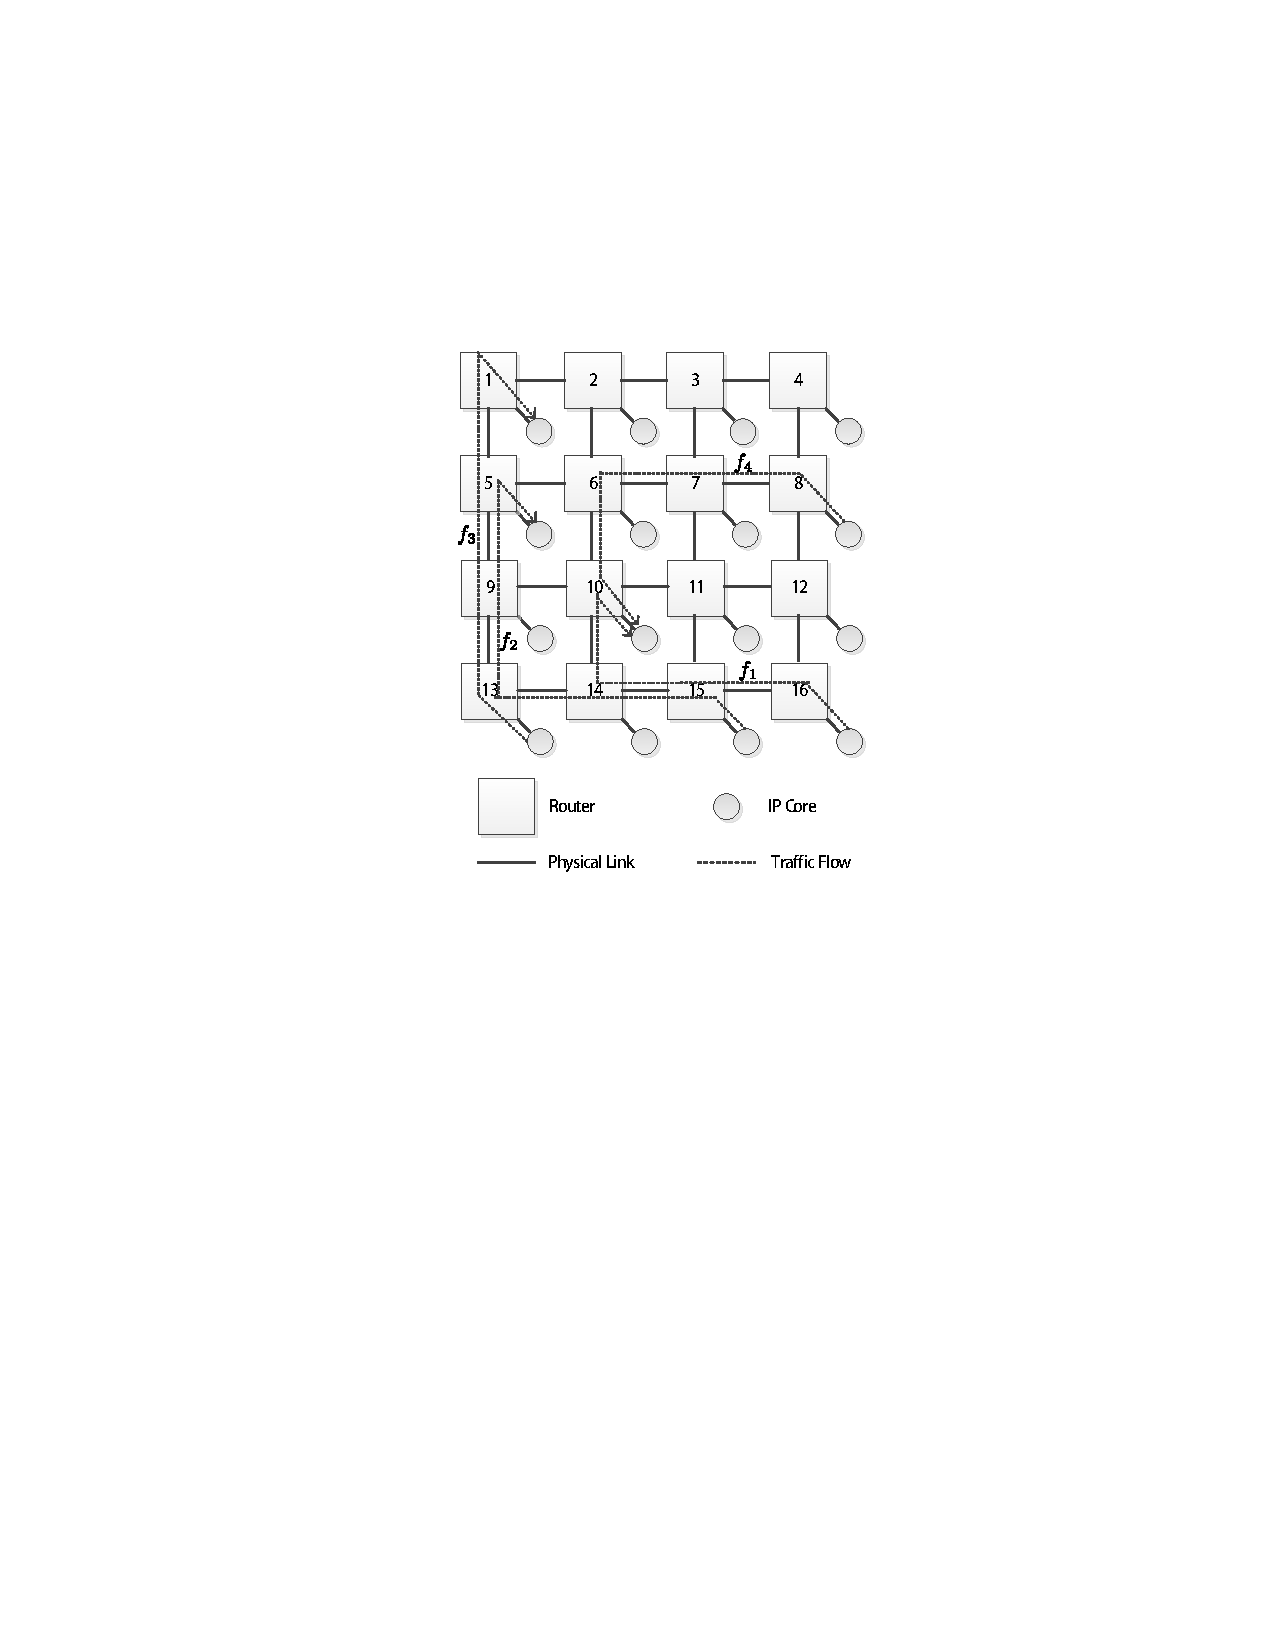
\includegraphics[scale=0.85]{figures/mesh.pdf}
  \caption{Mesh topology with four real-time traffic flows.}\label{topology}
\end{figure}

\subsection{Introduction to Real-Time Calculus}\label{intrortc}
Real-time calculus \cite{1253607} is the theoretic extension of the DNC theory \cite{Boudec2001Network}, by adding the upper service curve and lower arrival curve to describe the maximum service capability of a system and the minimum arrival rate of a event stream. It is the mathematical basis of the Modular Performance Analysis (MPA) \cite{Wandeler2006System} technique used for real-time task scheduling. Due to the space limitation, we only present the definitions of the RTC arrival curve and service curve in this subsection. For more details about this theory, please refer to \cite{1253607}.
\begin{rmk}[Real-Time Arrival Curve \cite{1253607}]\label{acu}
Denote by $R[s,t)$ the number of events arrived within the time interval $[s,t)$. The lower and upper bounds on $R[s,t)$ are called the lower arrival curve $\alpha^l$ and upper arrival curve $\alpha^u$, which satisfy
$$\alpha^l(t-s)\leq R[s,t)\leq \alpha^u(t-s),\forall s<t$$
and $\alpha^l(0)=\alpha^u(0)=0$. The RTC arrival curve for a event stream is denoted as $<\alpha^l,\alpha^u>$ for short.
\end{rmk}

\begin{rmk}[Real-Time Service Curve \cite{1253607}]
Denote by $S[s,t)$ the total number of events that can be processed by the system in the time interval $[s,t)$. The lower and upper bounds on $S[s,t)$ are called the lower service curve $\beta^l$ and upper service curve $\beta^u$, which satisfy
$$\beta^l(t-s)\leq S[s,t)\leq \beta^u(t-s),\forall s<t$$
and $\beta^l(0)=\beta^u(0)=0$. The RTC service curve for a system is denoted as $<\beta^l,\beta^u>$ for short.
\end{rmk}

From these two definitions, we find that the upper arrival curve and lower service curve correspond to the arrival curve and service curve of DNC theory \cite{Boudec2001Network}. Similarly, the upper service curve is identical to the maximum service curve of DNC theory. Thus, the two concatenation theorems for service curve (see Theorem 1.46 in \cite{Boudec2001Network}) and maximum service curve (see Theorem 1.6.1 in \cite{Boudec2001Network}) together form the concatenation theorem for the RTC service curve. Assume a event stream traverses two systems $S_1$ and $S_2$ in sequence, and $S_i$ offers an RTC service curve $<\beta^l_i,\beta^u_i>$ $(i=1,2)$ to this event stream. The concatenation theorem gives the equivalent RTC service curve offered by these two systems to this event stream, which is $<\beta^l_1\otimes\beta^l_2,\beta^u_1\otimes\beta^u_2>$.

In this paper, we will utilize the discrete time RTC arrival curve and service curve to characterize the arrived traffic and service capability of the wormhole-switched NoC, since the minimum time unit of this system is the clock period $T$. Events in the definitions of arrival curve and service curve refer to the arrival and service of flits, respectively. If we obtain the arrival curve $<\alpha^l,\alpha^u>$ of a specific flow at specific router and the service curve $<\beta^l,\beta^u>$ provided by this router, we can get the output arrival curve $<\alpha^{l^\prime},\alpha^{u^\prime}>$ of this flow and leftover service curve $<\beta^{l^\prime},\beta^{u^\prime}>$ of this router with the following equations \cite{1253607}:
\begin{equation}\label{alphal}
\alpha^{l^\prime}=\min\{(\alpha^l\oslash\beta^u)\otimes\beta^l,\beta^l\}
\end{equation}
\begin{equation}\label{alphau}
\alpha^{u^\prime}=\min\{(\alpha^u\otimes\beta^u)\oslash\beta^l,\beta^u\}
\end{equation}
\begin{equation}\label{betal}
\beta^{l^\prime}=(\beta^l-\alpha^u)\bar{\otimes}0
\end{equation}
\begin{equation}\label{betau}
\beta^{u^\prime}=\max\{(\beta^u-\alpha^l)\bar{\oslash}0,0\}
\end{equation}
where $\otimes$, $\oslash$, $\bar{\otimes}$, $\bar{\oslash}$ correspond to the min-plus convolution, min-plus de-convolution, max-plus convolution and max-plus de-convolution \cite{Boudec2001Network}.

After we obtain the arrival curve $<\alpha^l_{f},\alpha^u_{f}>$ of flow $f$ and the equivalent service curve $<\beta_{f}^l,\beta_{f}^u>$ offered by the system to flow $f$, we can get the end-to-end delay bound by the following equation \cite{Boudec2001Network}
\begin{equation}\label{delay}
Delay(f)=H(\alpha^u_{f},\beta^l_{f})
\end{equation}
where operator $H(\cdot,\cdot)$ means the maximal horizontal deviation between the two operands.

\section{Delay Analysis and Buffer Sizing}\label{modeling}
In this section, we first build an RTC based performance model for the priority-aware wormhole-switched NoC. Based on the constructed performance model, we then propose an end-to-end delay analysis algorithm and a buffer sizing algorithm.

The performance model comprises two parts, i.e. traffic model and service model. The traffic model utilizes the RTC arrival curve to describe the arrival process of each flow. We will introduce two methods to obtain the arrival curve in subsection \ref{traffic}. The service model characterize the services offered by the priority-aware NoC to each flow. The construction of service model is much more complicated than the traffic model. While constructing the service model, the follow three issues should be considered: (1) Only the head flit needs to traverse the RC and VA stages, because the non-head flits of a packet follow the data-path built by the head flit. To simplify our RTC model, we need a special mechanism to characterize the service offered to head and non-head flits in a unified way. (2) Our model extends the existing approach \cite{73}\cite{Qian489900} by allowing priority sharing among flows. Thus, the leftover service curve provided to the lower-priority flows can only be derived when all the service curves of high-priority flows have been computed. (3) We should first break the cyclic-dependence between the adjacent routers caused by flow control before analyzing the end-to-end delay bound with Eq.(\ref{delay}). We will discuss the first two issues in subsection \ref{sm}, and the last issue is discussed in subsection \ref{flowcontrol}. Finally, we present the delay analysis algorithm and buffer sizing algorithm in subsection \ref{e2elatency} and subsection \ref{bufferopt}, respectively.

\subsection{Traffic Model}\label{traffic}
The communication in a priority-aware wormhole-switched NoC is realized by transmitting packets, and the packet is further divided into flits, which is the minimum transmission unit in wormhole-switched NoC. Denote by $<\alpha^l(\Delta),\alpha^u(\Delta)>$ the flit arrival curve of a flow, namely, the minimum and maximum number of flits can be seen within any time window of length $\Delta$. We can extract the flit arrival curve from the synthetic traffic or communication trace with the sliding window method \cite{1253607}. For each window length $\Delta$, this method tries to find the maximal and minimal number of arrived flits (corresponding to $\alpha^l(\Delta)$ and $\alpha^u(\Delta)$) by analyzing the time series of flits. For the synthetic traffic or communication trace, the obtained arrival curve might not be periodic. But, it does not hinder the application of RTC theory, because the RTC arrival curve can characterize arbitrary traffic patterns.

However, the obtained flit arrival curve can only be applied to compute the worst-case performance bound at the flit level. To obtain the packet level delay bound, this arrival curve must be $L$-packetized \cite{Boudec2001Network}. Denote by $L(n)$ the cumulative packet length (in flits) of the first $n$ packets in a flow, $R(t)$ the cumulative arrived flits by time $t$. Then, the $L$-packetizer operator $\mathcal{P}^l(\cdot)$ is defined as $\mathcal{P}^L(R(t))=\underset{n\in\mathcal{N}}{\sup}\{L(n)1_{L(n)\leq R(t)}\}$\footnote{$\mathcal{N}$ is the set of natural numbers and $1_{\{val\}}$ is the indicator function, $1_{\{val\}}=1$ if and only if $val$ is true.}. Intuitively, $\mathcal{P}^l(\cdot)$ can be interpreted as the largest cumulative packet length contained in $R(t)$, as shown in Fig. \ref{lpkt}. For any flit arrival curve $<\alpha^l(\Delta),\alpha^u(\Delta)>$, the $L$-packetized arrival curve can be obtained by applying the following theorem.
\begin{thm}[$L$-packetized arrival curve]\label{pktac}
If a flow has a flit arrival curve $<\alpha^l(\Delta),\alpha^u(\Delta)>$, the flow also has a $L$-packetized arrival curve $<\alpha^l(\Delta)-l_{max}1_{\{\Delta>0\}},\alpha^u(\Delta)+l_{max}1_{\{\Delta>0\}}>$, where $l_{max}$ is the maximum packet length (in flits) of a flow.
\end{thm}
\begin{pf}
For $\forall t\geq 0,\Delta\geq 0$, according to the basic properties of $L$-packetizer \cite{Boudec2001Network}, we have
$$R(t)-l_{max}< \mathcal{P}^L(R(t))\leq R(t)$$
and
$$R(t+\Delta)-l_{max}< \mathcal{P}^L(R(t+\Delta))\leq R(t+\Delta).$$

The inequalities above indicate
$$R(t+\Delta)-R(t)-l_{max}< \mathcal{P}^L(R(t+\Delta))-\mathcal{P}^L(R(t))$$
and
$$\mathcal{P}^L(R(t+\Delta))-\mathcal{P}^L(R(t))< R(t+\Delta)-R(t)-l_{max}.$$

Based on the definition \ref{acu}, the $L$-packetized flow has a packet arrival curve $<\alpha^l(\Delta)-l_{max}1_{\{\Delta>0\}},\alpha^u(\Delta)+l_{max}1_{\{\Delta>0\}}>$.
which ends the proof.
\end{pf}

We can also directly obtain the $L$-packetized arrival curve instead of transformation from flit arrival curve for some special cases. For example, suppose all the packets in a flow have the same length $F$ and arrived periodically with period $I$. By applying the sliding window method \cite{1253607}, we can obtain the flit arrival curve of this flow, which is a pair of staircase functions\footnote{A staircase function $u_{T,\tau}=\lceil\frac{t+\tau}{T}\rceil$ for $t>0$ and 0 otherwise, where $0\leq \tau\leq T$ and $\lceil\cdot\rceil$ is the ceiling operator.} $<F\cdot u_{I,0},F\cdot u_{I,I}>$. As shown in Fig. \ref{perio}, the obtained flit arrival curve which is equal to the $L$-packetized arrival curve $\mathcal{P}^L(\alpha)$, since $\mathcal{P}^L(R(t))=R(t)$, $\mathcal{P}^L(\alpha^l(t))=\alpha^l(t)$ and $\mathcal{P}^L(\alpha^u(t))=\alpha^u(t)$.
\begin{figure*}
  \centering
  \subfloat[]{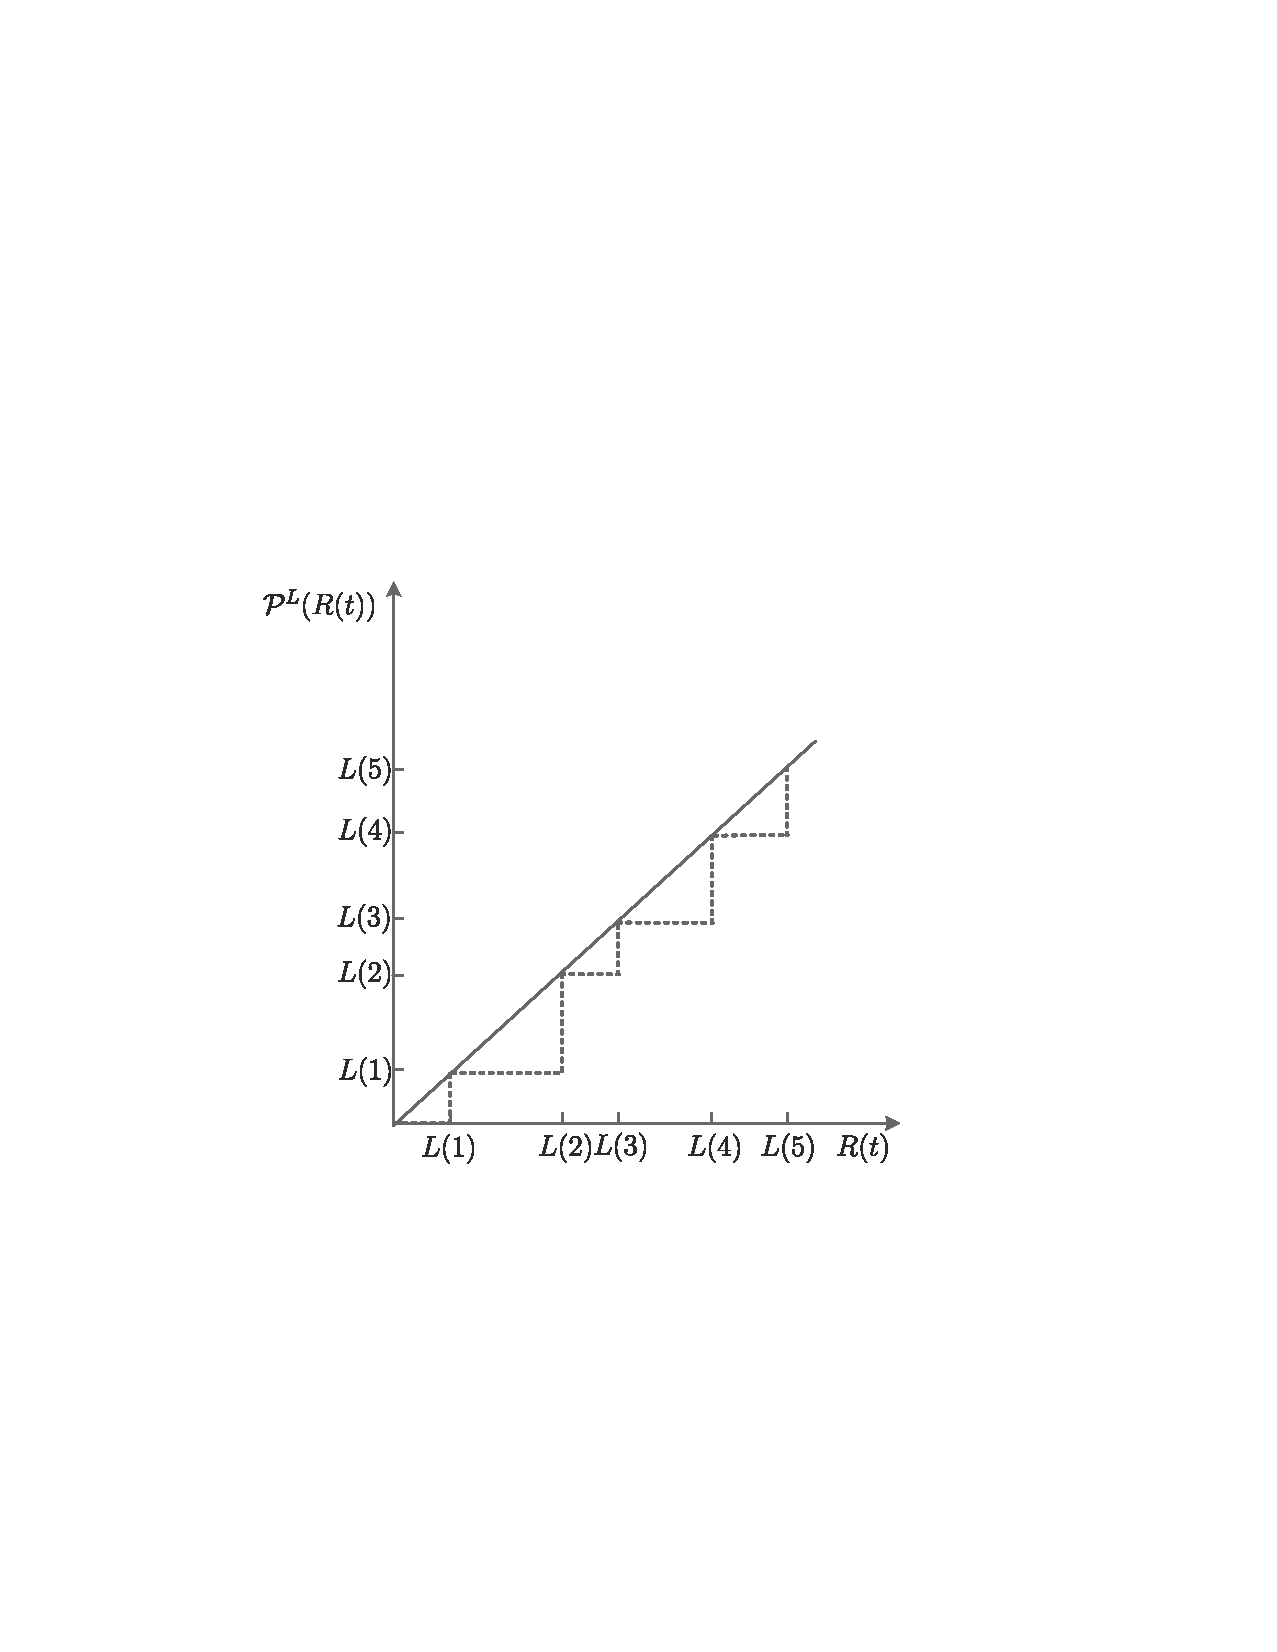
\includegraphics[scale=0.3]{figures/LPKT.pdf}\label{lpkt}}\hspace{10pt}
  \subfloat[]{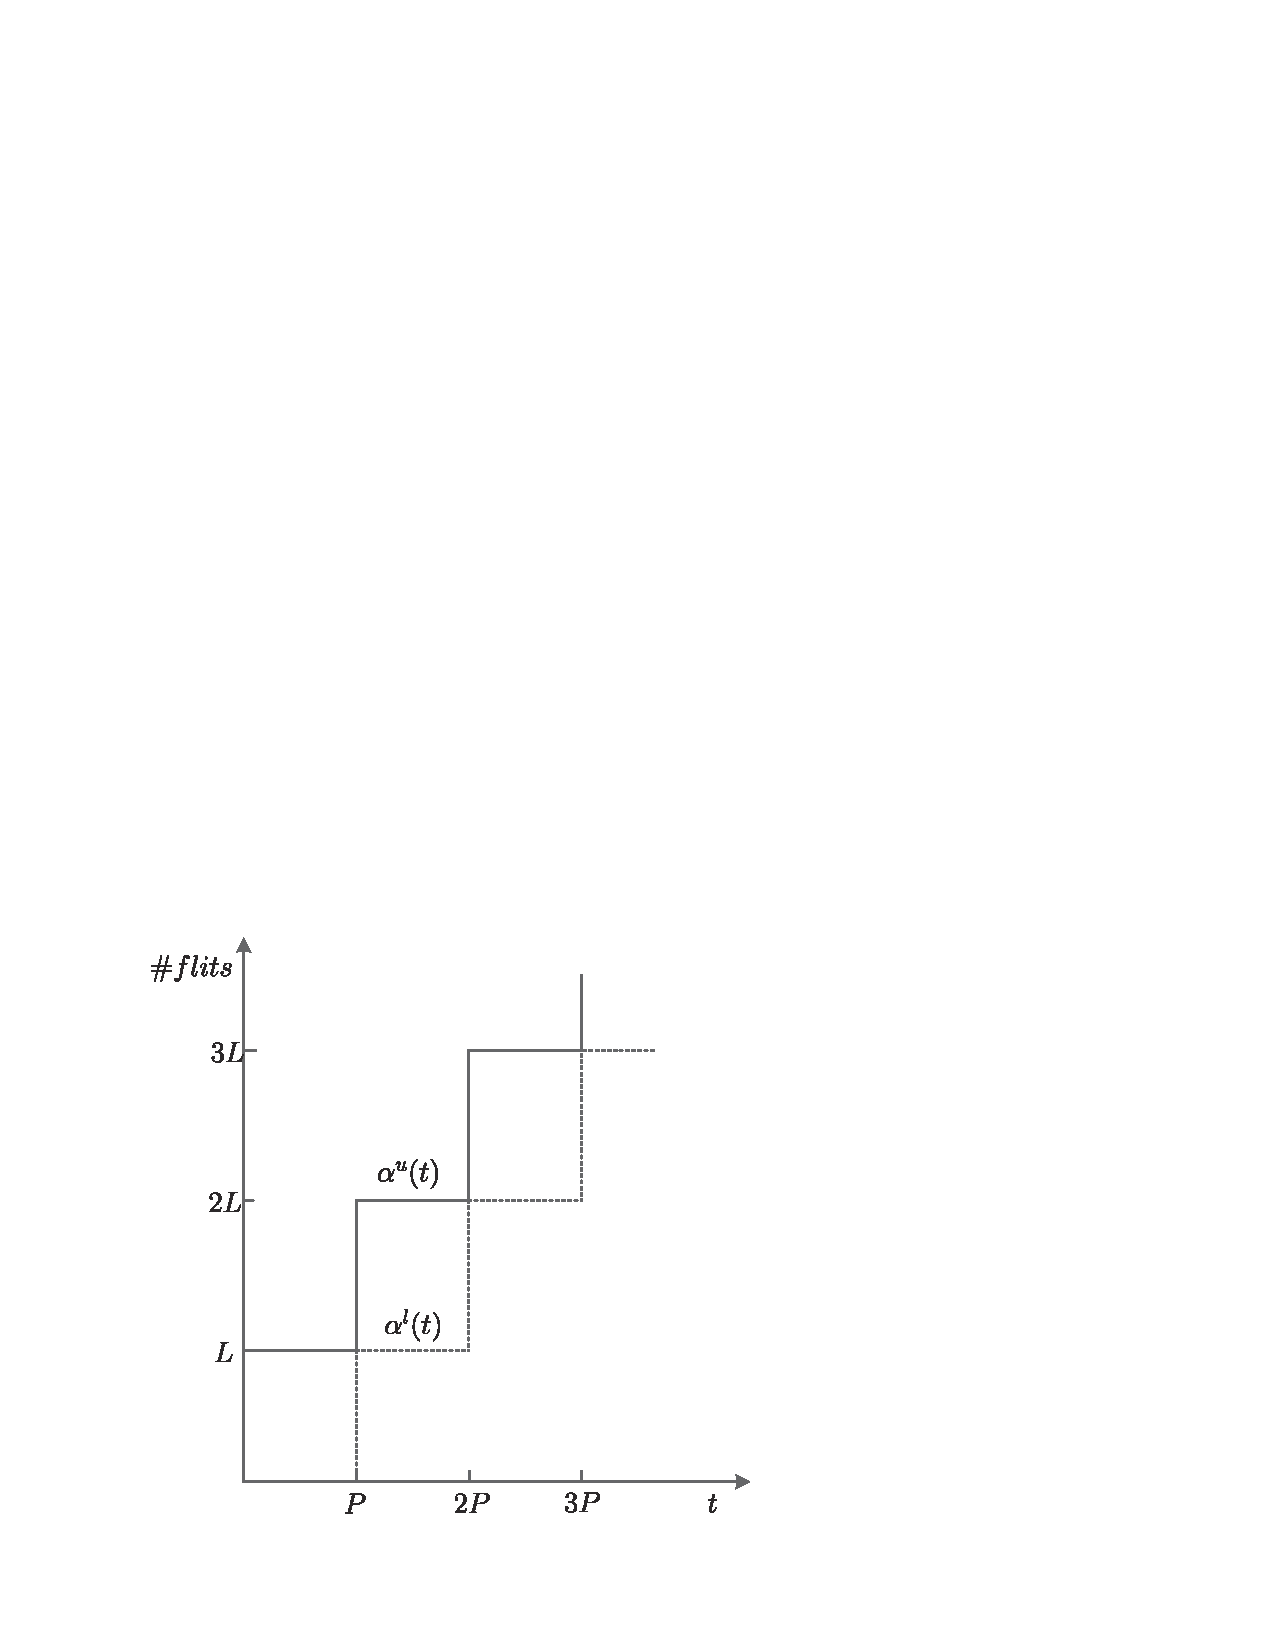
\includegraphics[scale=0.3]{figures/AC.pdf}\label{perio}}\hspace{10pt}
  \subfloat[]{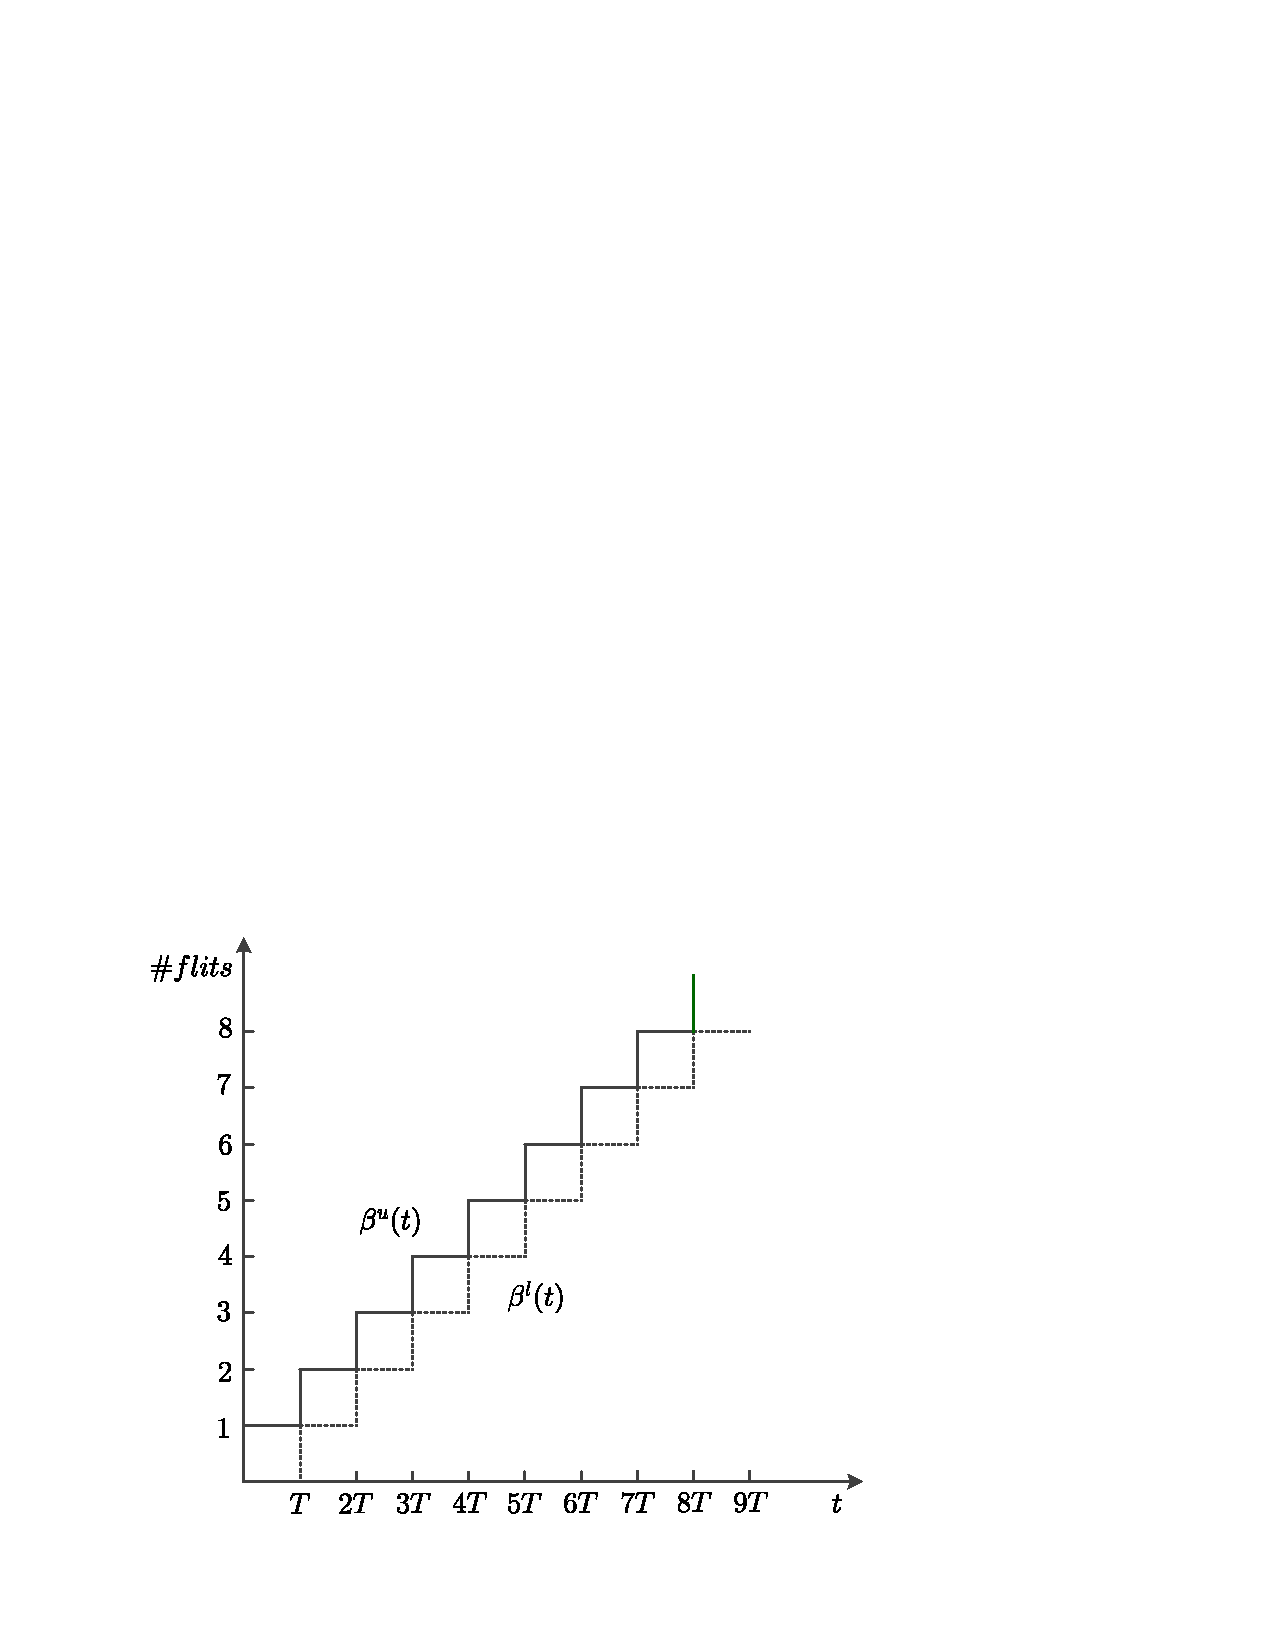
\includegraphics[scale=0.3]{figures/BW_ST_SA.pdf}\label{result1}}
  \caption{Traffic model and service model. (a) Definition of $\mathcal{P}^L(R(t))$. Cumulative arrival function $R(t)$ and the $L$-packetized cumulative arrival function $\mathcal{P}^L(R(t))$ are represented by the dotted line and solid line, respectively. (b) Real-time calculus arrival curve for periodically arrived traffic with period $I$ and packet length $F$. The solid line and dotted line represent the upper arrival curve and lower arrival curve. (c) Service model for each pipeline stage. The solid lines and dotted lines represent the upper service curves and lower service curves, respectively.}\label{ac}
\end{figure*}

\subsection{Basic Feed-forward Service Model}\label{sm}
The service model characterizes the service obtained by each flow at its source NI and entire path, which will be discussed as follows.

\subsubsection{Service Curve at Source NI}
If a IP core generates more than one flows simultaneously, the source NI will schedule these flows to go through the output link connecting the source NI and injection router according to their priorities. Figure \ref{ni} illustrates the internal structure of this priority-aware NI, where the IP core generates four flows simultaneously. Messages of different flows are encapsulated and stored in the dedicated buffer for that flow. The priority-aware scheduler selects one flit with the highest-priority at a time for transmission, and imposes an additional latency $T$ to all the flits which traverse it. Thus, the RTC service curve of the source NI (denoted as $<\beta^l_{NI},\beta^u_{NI}>$) can also be obtained by applying the sliding window method \cite{1253607}, as shown in Fig. \ref{result1}, which is a pair of staircase functions $<u_{T,0},u_{T,T}>$. Given the set of flow specifications, Algorithm \ref{alg:scatni} can derive the service curve obtained by each flow at the source NI. The flow specification of $f_i$ is a quadruple $(<\alpha^l,\alpha^u>,\mathcal{R}_i,D_i,P_i)$, which specifies the arrival curve, routine, deadline and priority of a flow.
\begin{figure}
  \centering
  % Requires \usepackage{graphicx}
  \includegraphics[scale=0.45]{figures/NI.pdf}
  \caption{Priority-aware NI. Each flow has its dedicated buffer, and the scheduler selects the flit with the highest-priority for transmission at each cycle.}\label{ni}
\end{figure}

\begin{algorithm}
\caption{Compute the service curve at source NI}\label{alg:scatni}
\begin{algorithmic}[1]
\Require The set of flow specifications
\Ensure The service curve obtained by each flow
\State Group the flows with priority $P_i$ into subset $\mathcal{F}_i$.
\State $\beta_{NI}^{l^\prime}=\lfloor\frac{t}{T}\rfloor$; $\beta_{NI}^{u^\prime}=\lceil\frac{t}{T}\rceil$.
\For {each $\mathcal{F}_i$ from highest priority to lowest priority}
    \For {each flow $f_j\in \mathcal{F}_i$}
        \State $\beta_{NI,f_j}^l=\lfloor\frac{\beta_{NI}^{l^\prime}}{|\mathcal{F}_i|}\rfloor$; //$|\mathcal{F}_i|$ denotes the cardinality of $\mathcal{F}_i$
        \State $\beta_{NI,f_j}^u=\lceil\frac{\beta_{NI}^{u^\prime}}{|\mathcal{F}_i|}\rceil$;
    \EndFor
    \State $\alpha^l=\sum_{f_j\in \mathcal{F}_i}\alpha^l_{f_j}$; $\alpha^u=\sum_{f_j\in \mathcal{F}_i}\alpha^u_{f_j}$;
    \State $\beta_{NI}^{l^\prime}=(\beta_{NI}^{l^\prime}-\alpha^u)\bar{\otimes}0$; $\beta_{NI}^{u^\prime}=\max\{(\beta_{NI}^{u^\prime}-\alpha^l)\bar{\oslash}0,0\}$;
\EndFor
\end{algorithmic}
\end{algorithm}

\subsubsection{Service Curve of a Router}\label{router}
While modeling the service capability of routers with RTC, we can analyze the data-path of a flow in a router stage-by-stage. On obtaining the service curves offered by each stage, the service curve provided by the router to a flow can be obtained by concatenating all the service curves of these stages. This is significantly different from the existing DNC based model \cite{qian2009analysis,Qian489900}, where they treat the entire router as a whole and designate a Latency-Rate (LR) service curve \cite{Boudec2001Network} to simplify the performance derivation. Whereas, our model uses the staircase functions to characterize the detailed behavior of this discrete time system. The advantage of our method is that, it can be easily modified to characterize the non-standard router micro-architectures, by simply letting the service curve of non-existed stages to be a burst delay function $\delta_0(t)$\footnote{$\delta_{val}(t)=+\infty$ if $t>val$, and 0 otherwise.}. Next, we try to derive the service curves of all these stages:

(1) BW stage, SA stage and LT stage: all the flits within a traffic flow will go through these three stages, and experience a fixed delay $T$ at each stage. The service curves provided by these stages, i.e. $<\beta^l_{BW},\beta^u_{BW}>$, $<\beta^l_{SA},\beta^u_{SA}>$ and $<\beta^l_{LT},\beta^u_{LT}>$, can be derived by applying the sliding window method \cite{1253607}, which are the same as the source NI, as shown in Fig. \ref{result1}.

(2) RC stage and VA stage: the latency of head flit experienced at these two stages is $T$. Although the non-head flits do not go through these two stages, they have to wait for two cycles before entering the SA stage at the worst-case, e.g. the three body flits of the same packet shown in Fig. \ref{pipeline}. Thus, a sophisticated solution to construct a unified lower service curve for head flit and non-head flits at these two stages comes from viewing each of these two stages impose an additional delay $T$ for all the flits. Thus, the equivalent lower service curve of these two stages, i.e. $\beta^l_{RC}$ and $\beta^l_{VA}$, can be easily obtained by the sliding window method \cite{1253607}, as shown in Fig. \ref{result1}. To derive the upper service curve of these two stages, let us consider the most `lucky' flits of a flow, e.g. the tail flit shown in Fig. \ref{pipeline}. This flit can enter the SA stage immediately after it was written into the dedicated VC buffer. For this case, the RC and VA stages impose a zero latency to it. Thus, we can utilize the burst delay function $\delta_0(t)$ to represent the upper service curve of these two stages.
\begin{figure}
  \centering
  \includegraphics[scale=0.35]{figures/Pipeline.pdf}
  \caption{Time-line graph of a packet going through the standard router pipeline. The delayed tail flit enters the ST stage immediately after it is written into the dedicated buffer.}\label{pipeline}
\end{figure}

(3) ST stage: each output port of the wormhole-switched NoC has a switch allocator to schedule the switch traversal among all the contending flows at each clock cycle. The notation $<\beta_{ST,R_i^{p}}^l,\beta_{ST,R_i^{p}}^u>$ is used to identify the service curve obtained by all the contending flows injected into switch port $p$. For the mesh topology, the port indicator $p$ can be concreted with $W$ (West port), $E$ (East port), $S$ (South port) and $N$ (North port) or $L$ (Local port). Thus, Following the same procedure as BW stage, we can get the service curves $<\beta_{ST,R_i^{p}}^l,\beta_{ST,R_i^{p}}^u>$, as shown in Fig. \ref{result1}.

Alert readers have noticed that, the contention of different flows within a router only occurs at ST stage. For the fixed-priority scheduling policy, switch allocators schedule the flow with the highest priority first, flows with the same priority will be served with Round-Robin order. All the unscheduled flows will be imposed an additional latency $T$ due to the failure of switch arbitration.

Denote by $<\beta_{ST,R_i^{p}}^l,\beta_{ST,R_i^{p}}^u>$ the total service curve provided by the ST stage, $<\beta_{ST,R_i,f_j}^l,\beta_{ST,R_i,f_j}^u>$ the service curve provided to flow $f_j$ by SA stage of router $R_i$, and $<\beta_{ST,R_i^{p}}^{l^\prime},\beta_{ST,R_i^{p}}^{u^\prime}>$ the leftover service curve after serving the flows with higher priority than $f_j$. In order to obtain the service curve $<\beta_{ST,R_i,f_j}^l,\beta_{ST,R_i,f_j}^u>$, we should consider the following two cases:

(a) All the flows contending with $f_j$ at $R_i$ have lower priorities. For the synchronized router architecture, flow $f_j$ gets the total leftover service curve $<\beta_{ST,R_i^{p}}^{l^\prime},\beta_{ST,R_i^{p}}^{u^\prime}>$.

(b) There exists some contention flows with the same priority as $f_j$. Since all the flows in $\Theta_{R_i,f_j}$ got serviced in Round-Robin order, the service curve provided to $f_j$ is $<\lfloor\beta^{l^\prime}_{ST,R_i^{p}}/(|\Theta_{R_i,f_j}|+1)\rfloor,\lceil\beta^{u^\prime}_{ST,R_i^{p}}/(|\Theta_{R_i,f_j}|+1)\rceil>$. After serving all the flows in $\Theta_{R_i,f_j}$, the leftover service curve for low-priority flows can be derived by applying Eq.(\ref{betal}) and Eq.(\ref{betau}).

After we obtained the service curve provided by ST stage to flow $f_j$, we can get the service curve of the router directly. The equivalent feed-forward service curve of router $R_i$ provided to $f_j$, i.e. $<\beta_{R_i,f_j}^l,\beta_{R_i,f_j}^u>$, can be obtained by concatenating the service curves of all these stages together:
$$\beta_{R_i,f_j}^l=\beta_{BW}^l\otimes\beta_{RC}^l\otimes\beta_{VA}^l\otimes\beta_{SA}^l\otimes \beta_{ST,R_i,f_j}^l,$$
$$\beta_{R_i,f_j}^u=\beta_{BW}^u\otimes\beta_{RC}^u\otimes\beta_{VA}^u\otimes\beta_{SA}^u\otimes \beta_{ST,R_i,f_j}^u.$$

\subsection{Feedback Service Model}\label{flowcontrol}
To this end, we have construct the traffic model and the feed-forward service model. Whereas, the credit-based flow control introduces cyclic-dependence between the adjacent routers, and leads to self-blocking within a flow due to the insufficiency of buffer space at the downstream router. The cyclic-dependence between the adjacent routers prevents us from deriving the performance bound directly even after we have obtained the service curve reserved at each router for the target flow. In existing literature, this cyclic-dependence is addressed by fixed-point iteration \cite{schioler2005network} or transformation from marked dataflow graph \cite{Thiele:2009:MPA:1629335.1629353}.

In this subsection, we will try to tackle the flow control problem with another solution motivated by \cite{qian2009analysis}, where the authors abstract the flow control as a network element (called flow controller) providing a service curve (corresponding to the lower service curve of RTC theory). Then, this service curve is obtained by applying some basic properties of DNC theory \cite{Boudec2001Network}. To make the discussion concrete, we take flow $f_2$ in Fig. \ref{topology} as an example and utilize the scheduling network model \cite{1253607} in RTC theory to visualize the credit-based flow control and complex relationship among $f_2$ and the other flows, as shown in Fig. \ref{f2}. We ignore flow $f_4$ and the flow control of the other flows for brevity and clarity. We also assume that, all the destination IP cores can consume the arrived flits immediately, thus there is no flow control between the ejection router and destination NI. However, to prevent the buffer overflow, the flow control between source NI and injection router is necessary.
\begin{figure*}
  \centering
  % Requires \usepackage{graphicx}
  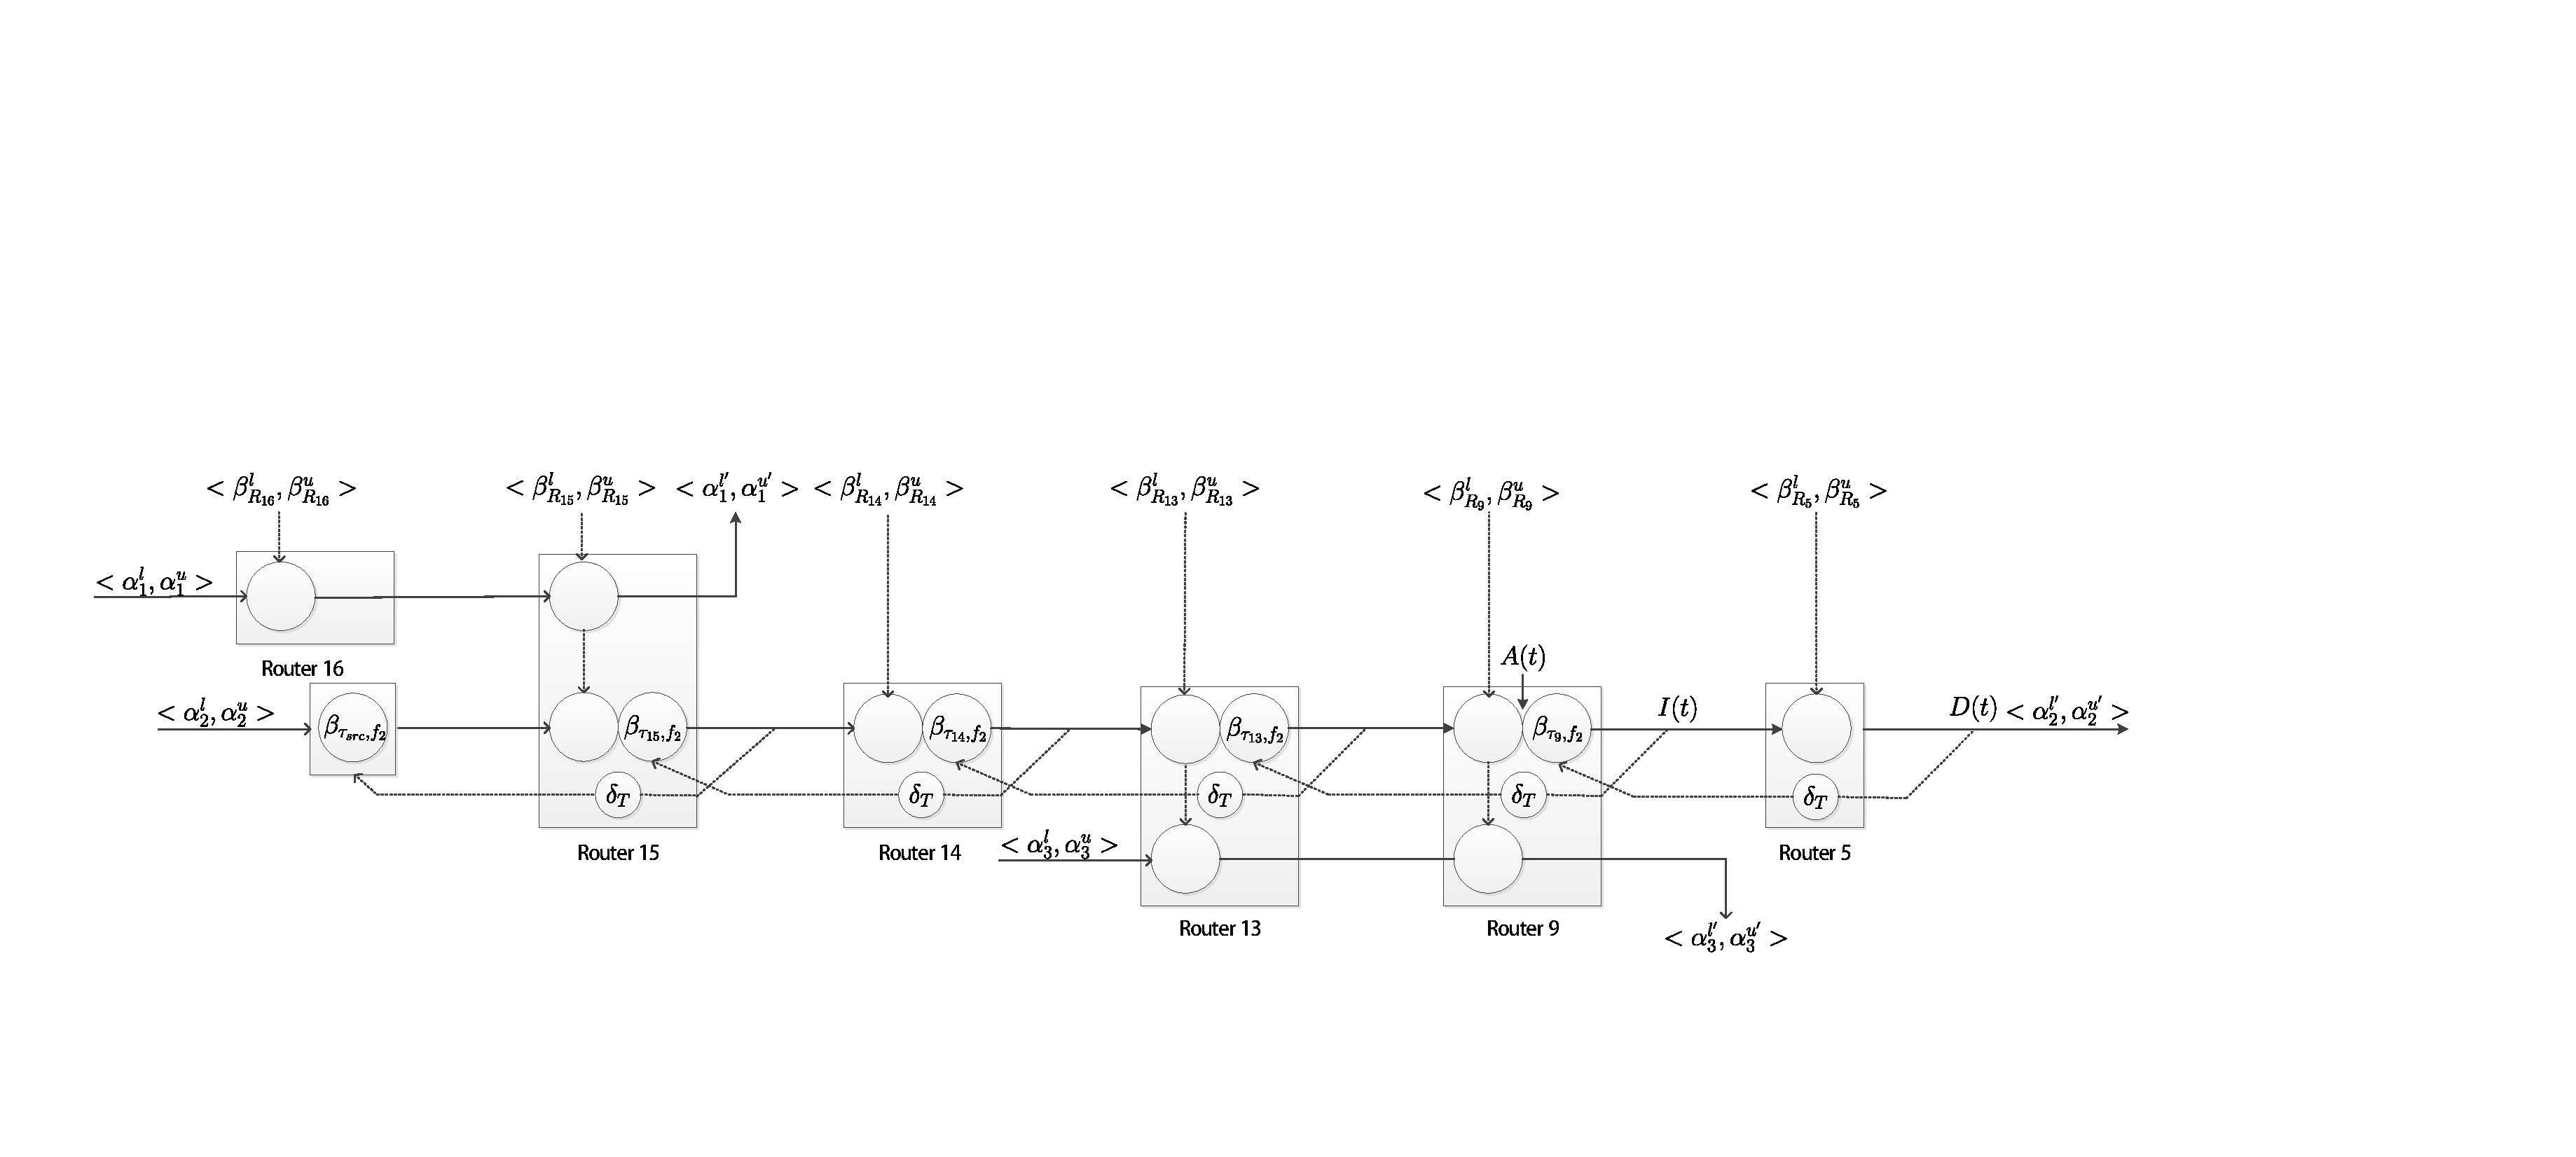
\includegraphics[scale=0.35]{figures/f2.pdf}\\
  \caption{Scheduling network model for flow $f_2$}\label{f2}
\end{figure*}

A flit in the wormhole router with credit-based flow control will be locked if the credits have been used up. We can abstract the blocking caused by credit-insufficiency as traversing a virtual pipeline stage, called Flow Control (FC) stage, as shown in Fig. \ref{f2}. The equivalent service curve for this virtual stage can be obtained by the following theorem, which enables us to break the cyclic-dependence caused by flow control and build a comprehensive performance model with RTC.
\begin{thm}\label{credit}
Suppose the physical link and router provide feed-forward service curve $<\beta_{LT}^l,\beta_{LT}^u>$ and $<\beta^l,\beta^u>$, the buffer size and credit feedback delay are denoted as $B$ and $\sigma$, respectively. Then, the flow controller provides an equivalent service curve $<\overline{\beta^l\otimes\beta_{LT}^l\otimes\delta_{\sigma}+B},\overline{\beta^u\otimes\beta_{LT}^u\otimes\delta_{\sigma}+B}>$, where $\bar{f}$ is the sub-additive closure \cite{Boudec2001Network} of $f$.
\end{thm}
\begin{pf}
We will take the flow control between $R_9$ and $R_5$ in Fig. \ref{f2} as an example to derive the service curve of flow controller. Denote the amount of injected and departed flits at $R_5$ by time $t$ as $I(t)$ and $D(t)$, and the amount of flits served by $R_9$ by time $t$ as $A(t)$. The feedback link can be represented as a network element providing upper service curve $\delta_\sigma(t)$. The DNC service curve (i.e. lower service curve of RTC) has been derived in \cite{qian2009analysis}, which is $\overline{\beta^l\otimes\beta_{LT}^l\otimes\delta_{\sigma}+B}$.

In the rest of this proof, we will only derive the upper service curve for the flow controller. For the flow control between router $R_9$ and $R_5$, we have $I(t)\leq A(t)$ for causality and $I(t)\leq D^\prime(t)+B$ due to the effect of flow control, where $D^\prime(t)\leq D\otimes\delta_\sigma(t)$. Thus, $$I(t)\leq\min\{A(t),D^\prime(t)+B\}.$$

Based on the equivalent definition of upper service curve\footnote{please refer to definition 1.6.1 in \cite{Boudec2001Network} for more details.}, we have
$$D(t)\leq I\otimes \beta_{R_5,f_2}^u\otimes\beta_{LT}^u(t).$$

Bring $I(t)$ and $D^\prime(t)$ into this equality, we get
\begin{eqnarray*}
D(t)&\leq& I\otimes \beta_{R_5,f_2}^u\otimes\beta_{LT}^u(t)\\
&\leq& \min\{A\otimes \beta^u_{R_5,f_2}\otimes\beta_{LT}^u(t),D\otimes\delta_\sigma\otimes \beta_{R_5,f_2}^u\otimes\beta_{LT}^u(t)+B\}.
\end{eqnarray*}

By applying Theorem 4.31 in \cite{Boudec2001Network}, we have
$$D\leq A\otimes \beta^u_{R_5,f_2}\otimes\beta_{LT}^u\otimes\overline{\beta_{R_5,f_2}^u\otimes\beta_{LT}^u\otimes\delta_\sigma+B}.$$

Thus,
\begin{eqnarray*}
  I&\leq& \min\{A,D^\prime+B\}\\
  &\leq& \min\{A,D\otimes\delta_\sigma+B\}\\
  &\leq& \min\{A,A\otimes \beta^u_{R_5,f_2}\otimes\beta_{LT}^u\otimes\overline{\beta_{R_5,f_2}^u\otimes\beta_{LT}^u\otimes\delta_\sigma+B}\otimes\delta_\sigma+B\}\\
%  &=& \min\{A\otimes \delta_\sigma,A\otimes (\beta_{R_5^L,f_2}^u\otimes\delta_\sigma+B)\otimes\overline{\delta_\sigma\otimes\beta_{R_5^L,f_2}^u+B}\}\\
  &=& \min\{A\otimes \delta_\sigma,A\otimes \overline{\delta_\sigma\otimes\beta_{R_5,f_2}^u\otimes\beta_{LT}^u+B}\}\\
  &=& A\otimes\min\{\delta_\sigma,\overline{\beta_{R_5,f_2}^u\otimes\beta_{LT}^u\otimes\delta_\sigma+B}\}\\
  &=& A\otimes\overline{\beta_{R_5,f_2}^u\otimes\beta_{LT}^u\otimes\delta_\sigma+B}
\end{eqnarray*}
where the steps from the third line to the fifth line hold due to the general properties of $\otimes$ operator (see Rule 6 and Rule 7 of Theorem 3.1.5 in \cite{Boudec2001Network} for more details), and the last step follows from the definition of sub-additive closure.

The inequality $I\leq A\otimes \overline{\beta_{R_5,f_2}^u\otimes\beta_{LT}^u\otimes\delta_\sigma+B}$ implies that the flow controller between $R_9$ and $R_5$ provides an upper service curve $\overline{\beta_{R_5,f_2}^u\otimes\beta_{LT}^u\otimes\delta_\sigma+B}$. Thus, we can conclude that for any router providing upper service curve $\beta^u$, the corresponding flow controller offers an upper service curve $\overline{\beta^u\otimes\beta_{LT}^u\otimes\delta_\sigma(t)+B}$.
\end{pf}

On obtaining the equivalent service curve of flow controller for $f_i$ at router $R_j$ (denoted as $<\beta_{FC,R_j,f_i}^l,\beta_{FC,R_j,f_i}^u>$), we get the equivalent service curve of router $R_j$ after breaking the cyclic-dependence loop:
$$\beta_{R_j,f_i}^l=\beta_{BW}^l\otimes\beta_{RC}^l\otimes\beta_{VA}^l\otimes\beta_{SA}^l\otimes\beta_{ST,R_j,f_i}^l\otimes\beta_{FC,R_j,f_i}^l,$$
$$\beta_{R_j,f_i}^u=\beta_{BW}^u\otimes\beta_{RC}^u\otimes\beta_{VA}^u\otimes\beta_{SA}^u\otimes\beta_{ST,R_j,f_i}^u\otimes\beta_{FC,R_j,f_i}^u.$$

Theorem \ref{credit} derives the RTC service curve of a single flow controller, and we can get the service curves of all the flow controllers along the router chain of any flow by applying Theorem \ref{credit} iteratively. As shown in Fig. \ref{f2}, the service curve of a flow controller is determined by the service curves of the downstream flow controllers and routers. Hence, for each flow, we should compute the service curves of flow controllers from the ejection router to the injection router. Take flow $f_2$ as an example, we have $\beta_{FC,R_5,f_2}^l(t)=\delta_0(t)$ and $\beta_{FC,R_5,f_2}^u(t)=\delta_0(t)$ since there is no flow control between $R_5$ and destination NI. Then, we compute the service curve of flow controller between $R_5$ and $R_{9}$ (i.e. $<\beta_{FC,R_9,f_2}^l,\beta_{FC,R_9,f_2}^u>$), which is $<\overline{\beta_{R_5,f_2}^l\otimes\beta_{LT}^l\otimes\delta_\sigma+B},\overline{\beta_{R_5,f_2}^u\otimes\beta_{LT}^u\otimes\delta_\sigma+B}>$. By applying the concatenation theorem, we can obtain the equivalent service curve provided to $f_2$ by router $R_{9}$, which can be utilized to derive $<\beta_{FC,R_{13},f_2}^l,\beta_{FC,R_{13},f_2}^u>$ further. Following the same procedure, the service curve $<\beta_{FC,R_{14},f_2}^l,\beta_{FC,R_{14},f_2}^u>$, $<\beta_{FC,R_{15},f_2}^l,\beta_{FC,R_{15},f_2}^u>$ and $<\beta_{FC,NI,f_2}^l,\beta_{FC,NI,f_2}^u>$\footnote{$<\beta_{FC,NI,f_2}^l,\beta_{FC,NI,f_2}^u>$ denotes the service curve of flow controller between source NI and injection router.} can be derived iteratively.

\subsection{End-to-End Delay Analysis}\label{e2elatency}
In this subsection, we present the delay analysis algorithm, as shown in Algorithm \ref{alg:equivalentservicecurve}. This algorithm takes the architecture parameters and flow specifications as input, and gives the worst-case end-to-end delay for all the flows. The architecture parameters specify the network topology graph,buffer size of each VC and the service curve of each pipeline stage. The flow specifications specifies the arrival curve, routine, deadline and priority of each flow.

In this algorithm, the arrival curve of flow $f_i$ at the source NI and router $R_j$ are denoted as $<\alpha_{f_i}^l,\alpha_{f_i}^u>$ and $<\alpha_{R_j,f_i}^l,\alpha_{R_j,f_i}^u>$, respectively. The leftover service curve of ST stage at output port $p$ is represented as $<\beta_{ST,R_j^{p}}^{l^\prime},\beta_{ST,R_j^{p}}^{u^\prime}>$ (Initially, let $\beta_{ST,R_j^{p}}^{l^\prime}=\beta_{ST,R_j^{p}}^{l}$ and $\beta_{ST,R_j^{p}}^{u^\prime}=\beta_{ST,R_j^{p}}^{u}$). In the fixed-priority flit-level preemptive NoC, only the leftover service curve can be used by the low-priority flows. Thus, our algorithm compute the leftover service curve and delay bound from high-priority flows to low-priority flows. For each iteration, it performs the following four steps in sequence: (1) Calculating the service curves provided by the routers (lines 4-5) and flow controllers (lines 6-7) along the path. (2) Computing the worst-case end-to-end delay of the flow (lines 9-11), where the service curve provided by the source NI to $f_i$, i.e. $<\beta_{NI,f_i}^l,\beta_{NI,f_i}^u>$ has been computed with Algorithm \ref{alg:scatni}. (3) The highlights of performance model when compared with the LLA method \cite{73} and DNC method \cite{Qian489900} is that our algorithm supports the priority-sharing. Thus, the leftover service curve at each router for low-priority flows can only be calculated when all the flows sharing the same priority have been calculated. To calculate the leftover service curve at ST stage, we have to first derive the equivalent service curve from source NI to $R_j$ (lines 15-16) and the arrival curve at $R_j$ (lines 17-18). Then, derive the leftover service curve with the aggregate arrival curve of the same priority-level (lines 20-23). The overall algorithm has two-level embedded loops, and the computation complexity for this algorithm is $O(HN)$, where $N$ and $H$ is the number of flows and the hop count of each flow. This algorithm can be easily integrated into the RTC toolbox \cite{rtc} to compute the end-to-end delay bound automatically. Since our algorithm takes the maximum service capability and minimum service rate into consideration, our algorithm can give much tighter delay bound than the DNC-based delay analysis algorithm proposed in \cite{Qian489900}.
\begin{algorithm}
\caption{End-to-end delay analysis algorithm}
\label{alg:equivalentservicecurve}
\begin{algorithmic}[1]
\Require Architecture parameters and flow specifications
\Ensure Worst-case end-to-end delay for all the flows
    \For {each flow $f_i\in \mathcal{F}$ with priority order}
        \State $\beta_{\tau}^l=\delta_0(t)$; $\beta_{\tau}^u=\delta_0(t)$;
        \For {each router $R_j\in \mathcal{R}_{i}$ from $end_i$ to $start_i$}
            \State $\beta_{R_j,f_i}^l=\beta_{BW}^l\otimes\beta_{RC}^l\otimes\beta_{VA}^l\otimes\beta_{SA}^l\otimes\lfloor\frac{\beta_{ST,R_j^{p}}^{l^\prime}}{|\Theta_{R_j,f_i}|+1}\rfloor\otimes\beta_{\tau}^l$;
            \State $\beta_{R_j,f_i}^u=\beta_{BW}^u\otimes\beta_{RC}^u\otimes\beta_{VA}^u\otimes\beta_{SA}^u\otimes\lceil\frac{\beta_{ST,R_j^{p}}^{u^\prime}}{|\Theta_{R_j,f_i}|+1}\rceil\otimes\beta_{\tau}^u$;
            \State $\beta_{\tau}^l=\overline{\beta^l_{R_j,f_i}\otimes\beta_{LT}^l\otimes\delta_\sigma(t)+B_{R_j,f_i}}$;
            \State $\beta_{\tau}^u=\overline{\beta^u_{R_j,f_i}\otimes\beta_{LT}^u\otimes\delta_\sigma(t)+B_{R_j,f_i}}$;
        \EndFor
        \State $\beta_{FC,NI,f_i}^l=\beta^l_{\tau}$; $\beta_{FC,NI,f_i}^u=\beta^u_{\tau}$;
        \State $\beta_{f_i}^l=\beta_{NI,f_i}^l\otimes\beta_{FC,NI,f_i}^l\otimes (\underset{R_k\in\mathcal{R}_{i}}{\otimes}(\beta^l_{R_k,f_i}\otimes\beta^l_{LT}))$;
        \State $Delay(f_i)=H(\alpha^u_{f_i},\beta_{f_i}^l)$;
    \EndFor
\end{algorithmic}
\end{algorithm}

\begin{algorithm}
\caption{Compute the leftover service curve at ST stage after serving}
\label{alg:leftoverscl}
\begin{algorithmic}[1]
\Require $<\alpha_{f_i}^l,\alpha^u_{f_i}>$, $<\beta_{NI,f_i}^l,\beta_{NI,f_i}^u>$ and $<\beta_{R_j,f_i}^l,\beta_{R_j,f_i}^u>$.
\Ensure Leftover service curve at ST stage
\Function{$Leftover\_Service\_Curve$}{$a$}
\State $\beta_{f_i}^l=\beta_{NI,f_i}^l\otimes\beta_{FC,NI,f_i}^l$; $\beta_{f_i}^u=\beta_{NI,f_i}^u\otimes\beta_{FC,NI,f_i}^u$;
\For {$\forall R_j\in\mathcal{R}_{i}$ from $start_i$ to $end_i$}
    \If {$\Omega_{R_j,f_i}\neq \emptyset$}
        \State $\beta^l=\beta^l_{f_i}\otimes\beta_{BW}^l\otimes\beta_{RC}^l\otimes\beta_{VA}^l\otimes\beta_{SA}^l$;
        \State $\beta^u=\beta^u_{f_i}\otimes\beta_{BW}^u\otimes\beta_{RC}^u\otimes\beta_{VA}^u\otimes\beta_{SA}^u$;
        \State $\alpha^l_{R_j,f_i}=\min\{(\alpha^l_{f_i}\oslash\beta^u)\otimes\beta^l,\beta^l\}$;
        \State $\alpha^u_{R_j,f_i}=\min\{(\alpha^u_{f_i}\otimes\beta^u)\oslash\beta^l,\beta^u\}$;
        \If {$\forall f_k\in\Theta_{R_j,f_i}$ have been calculated}
            \State $\alpha^l_{R_j,f_i}=\alpha^l_{R_j,f_i}+\sum_{f_k\in\Theta_{R_j,f_i}}\alpha^l_{R_j,f_k}$;
            \State $\alpha^u_{R_j,f_i}=\alpha^u_{R_j,f_i}+\sum_{f_k\in\Theta_{R_j,f_i}}\alpha^u_{R_j,f_k}$;
            \State $\beta^{l^\prime}_{ST,R_j^{p}}=(\beta^{l^\prime}_{ST,R_j^{p}}-\alpha^u_{R_j,f_i})\bar{\otimes}0$;
            \State $\beta^{u^\prime}_{ST,R_j^{p}}=\max\{(\beta^{u^\prime}_{ST,R_j^{p}}-\alpha^l_{R_j,f_i})\bar{\oslash}0,0\}$;
        \EndIf
    \EndIf
    \State $\beta_{f_i}^l=\beta_{f_i}^l\otimes\beta^l_{R_j,f_i}$; $\beta_{f_i}^u=\beta_{f_i}^u\otimes\beta^u_{R_j,f_i}$;
    \State \Return $<\beta^{l^\prime}_{ST,R_j^{p}},\beta^{u^\prime}_{ST,R_j^{p}}>$;
\EndFor
\EndFunction
\end{algorithmic}
\end{algorithm}

\subsection{Buffer Sizing}\label{bufferopt}
The priority-aware wormhole-switched NoC \cite{Shi:2008:RCA:1397757.1397996,708526,627905} requires the same amount of VCs as the priorities to prevent priority inversion, which refers to the blocking of high-priority flows when the low priority flows occupy all the VCs \cite{707545}. To reduce the buffer area and power consumption of priority-aware wormhole-switched NoC, priority sharing \cite{5161497} and buffer optimization \cite{189} techniques have been proposed. However, the backlog bound derived in \cite{189} is the minimum buffer size that does not trigger the flow control. Reducing this buffer size further will cause the back-pressure between adjacent routers and leads to a larger end-to-end delay. However, it is allowed to do so as long as the deadline constraint of each flow is not being violated. Our buffer sizing algorithm reduces the initial buffer size iteratively as long as the end-to-end delay of a flow is less than its deadline and the buffer size is greater than one. The initial buffer size to avoid flow control can be obtained by the follow theorem.
\begin{thm}
Denote by $\beta_{R_j,f_i}^l$ the feed-forward lower service curve obtained at $R_j\in\mathcal{R}_i$ by flow $f_i$, $\beta_{LT}^l$ the lower service curve provided by the physical link between two adjacent routers, $B_{R_j,f_i}$ the VC buffer size reserved for $f_i$ at $R_j$ and $\sigma$ the credit feedback delay. Then, the buffer size at each router $R_j\in\mathcal{R}_i$ to avoid flow control is $$B_{R_j,f_i}=\lceil\inf\{B|\beta_{R_j,f_i}^l\otimes\beta_{LT}^l\otimes\overline{\beta_{R_j,f_i}^l\otimes\beta_{LT}^l\otimes\delta_\sigma(t)+B}\geq\beta_{R_j,f_i}^l\otimes\beta_{LT}^l\}\rceil.$$
\end{thm}
\begin{pf}
We take flow $f_2$ in Fig. \ref{topology} as an example to prove this theorem. As stated by Theorem \ref{credit}, $$\beta_{FC,R_9,f_2}^l=\overline{\beta^l_{LT}\otimes\beta_{R_5,f_2}^l\otimes\delta_\sigma+B_5},$$
\begin{eqnarray}
\beta_{FC,R_{13},f_2}^l&=&\overline{\beta^l_{LT}\otimes\beta^l_{R_9,f_2}\otimes\overline{\beta^l_{LT}\otimes\beta^l_{R_5,f_2}\otimes\delta_\sigma+B_5}\otimes\delta_\sigma+B_9}\label{eq1}\\
&=&\overline{(\beta^l_{LT}\otimes\beta^l_{R_9,f_2}+B_9)\otimes\delta_\sigma\otimes\overline{(\beta^l_{LT}\otimes\beta^l_{R_5,f_2}+B_5)\otimes\delta_\sigma}}\label{eq2}\\
&=&\overline{(\beta^l_{LT}\otimes\beta^l_{R_9,f_2}+B_9)\otimes\delta_\sigma}\otimes\overline{(\beta^l_{LT}\otimes\beta^l_{R_5,f_2}+B_5)\otimes\delta_\sigma}\label{eq3}
\end{eqnarray}
where the step from line \ref{eq1} to line \ref{eq2} holds due to the basic property of min-plus convolution (see Rule 7 of Theorem 3.1.5 in \cite{Boudec2001Network}). By Theorem 3.1.11 in \cite{Boudec2001Network}, the last line holds.

Similarly, $$\beta_{FC,R_{14},f_2}^l=\overline{(\beta^l_{LT}\otimes\beta^l_{R_{13},f_2}+B_{13})\otimes\delta_\sigma}\otimes\beta_{FC,R_{13},f_2}^l,$$
$$\beta_{FC,R_{15},f_2}^l=\overline{(\beta^l_{LT}\otimes\beta^l_{R_{14},f_2}+B_{14})\otimes\delta_\sigma}\otimes\beta_{FC,R_{13},f_2}^l,$$
$$\beta_{FC,NI,f_2}^l=\overline{(\beta^l_{LT}\otimes\beta^l_{R_{15},f_2}+B_{15})\otimes\delta_\sigma}\otimes\otimes\beta_{FC,R_{13},f_2}^l.$$

Then, the equivalent feedback service curve obtained by $f_2$ is
\begin{eqnarray}
\beta_{f_2}^l&=&\beta_{NI,f_2}^l\otimes\beta_{FC,NI,f_2}^l\otimes(\underset{R_j\in\mathcal{R}_i}{\otimes}\beta^l_{R_j,f_i}\otimes\beta^l_{FC,R_j,f_i}\otimes\beta_{LT}^l)\\
&=& \beta_{NI,f_2}^l\otimes(\underset{R_j\in\mathcal{R}_i}{\otimes}\beta^l_{R_j,f_i}\otimes\beta_{LT}^l\otimes\overline{(\beta^l_{LT}\otimes\beta^l_{R_{j},f_2}+B_{R_j,f_2})\otimes\delta_\sigma})
\end{eqnarray}
where the last two steps hold due to the commutativity of min-plus convolution and the basic property of sub-additive closure (see Corollary 3.1.1 in \cite{Boudec2001Network}).

According to the isotonicity of min-plus convolution (see Theorem 3.1.7 in \cite{Boudec2001Network}), we know that $$\beta_{R_j,f_i}^l\otimes\beta_{LT}^l\otimes\overline{\beta_{R_j,f_i}^l\otimes\beta_{LT}^l\otimes\delta_\sigma(t)+B}\geq\beta_{R_j,f_i}^l\otimes\beta_{LT}^l,\forall R_j\in\mathcal{R}_i$$ is a sufficient condition for avoiding flow control, which ends the proof.
\end{pf}

Suppose the applications have been mapped onto the NoC, and each flow $f_i$ has been assigned to their corresponding priority $P_i$ and deadline $D_i$. Following the same notation as Algorithm 1, we propose the buffer sizing algorithm to allocate just enough buffer for each flow to meet their deadline constraint, as shown in Algorithm \ref{alg:bufopt}. It tries to reduce the buffer size for each flow from high-priority to low-priority gradually. For each iteration, it performs the following four steps: (1) Calculating the service curves provided by the routers (lines 3-5). Initially, we set the service curves of all the flow controllers to be $<\delta_0(t),\delta_0(t)>$, because the initial buffer is large enough to avoid flow control. (2) Calculate the minimum buffer size that can avoid flow control for each router (lines 6-8). (3) Reduce the initial buffer size gradually as long as the constraint of deadline is not being violated (lines 10-26), where the service curve provided by the source NI of $f_i$,i.e. $<\beta_{NI,f_i}^l,\beta_{NI,f_i}^u>$, has been computed with Algorithm \ref{scatni}. (4) Calculating the leftover service curve at each router for low-priority flows (lines 27-42). This algorithm can be implemented in RTC toolbox \cite{rtc} to optimize the buffer size automatically.
\begin{algorithm}
\caption{Buffer sizing algorithm}
\label{alg:bufopt}
\begin{algorithmic}[1]
\Require Architecture parameters and flow specifications
\Ensure Optimized buffer size
    \For {each flow $f_i\in \mathcal{F}$ with priority order}
        \For {each router $R_j\in \mathcal{R}_{i}$}
            \State $\beta_{R_j,f_i}^l=\beta_{BW}^l\otimes\beta_{RC}^l\otimes\beta_{VA}^l\otimes\beta_{SA}^l\otimes\lfloor\frac{\beta_{ST,R_j^{p}}^{l^\prime}}{|\Theta_{R_j,f_i}|+1}\rfloor$;
            \State $\beta_{R_j,f_i}^u=\beta_{BW}^u\otimes\beta_{RC}^u\otimes\beta_{VA}^u\otimes\beta_{ST}^u\otimes\lceil\frac{\beta_{ST,R_j^{p}}^{u^\prime}}{|\Theta_{R_j,f_i}|+1}\rceil$;
            \State $B_{R_j,f_i}=\lceil\inf\{B|\beta_{R_j,f_i}^l\otimes\beta_{LT}^l\otimes\overline{\beta_{R_j,f_i}^l\otimes\beta_{LT}^l\otimes\delta_\sigma+B}\geq\beta_{R_j,f_i}^l\otimes\beta_{LT}^l\}\rceil$;
        \EndFor
        \State $\beta_{FC,NI,f_i}^l=\delta_0(t)$; $\beta_{FC,NI,f_i}^u=\delta_0(t)$;
        \For {each router $R_j\in \mathcal{R}_{i}$ from $end_i$ to $start_i$}
            \State $\beta_{f_i}^l=\beta_{NI,f_i}^l\otimes\beta_{FC,NI,f_i}^l\otimes(\underset{R_k\in\mathcal{R}_{i}}{\otimes}(\beta^l_{R_k,f_i}\otimes\beta^l_{LT}))$;
            \While {$H(\alpha^u_{f_i},\beta_{f_i}^l)\leq D_i$ and $B_{R_j,f_i}>1$}
                \State $B_{R_j,f_i}=B_{R_j,f_i}-1$;
                \State $\beta_\tau^l=\beta_{FC,R_j,f_i}^l$; $\beta_\tau^u=\beta_{FC,R_j,f_i}^u$;
                \For {all $R_{k}$ from $R_j$ to $start_i$}
                    \State $\beta_{R_k,f_i}^l=\beta_{BW}^l\otimes\beta_{RC}^l\otimes\beta_{VA}^l\otimes\beta_{SA}^l\otimes\lfloor\frac{\beta_{ST,R_k^{p}}^{l^\prime}}{|\Theta_{R_k,f_i}|+1}\rfloor\otimes\beta_{\tau}^l$;
                    \State $\beta_{R_k,f_i}^u=\beta_{BW}^u\otimes\beta_{RC}^u\otimes\beta_{VA}^u\otimes\beta_{ST}^u\otimes\lceil\frac{\beta_{ST,R_k^{p}}^{u^\prime}}{|\Theta_{R_k,f_i}|+1}\rceil\otimes\beta_{\tau}^u$;
                    \State $\beta_{\tau}^l=\overline{\beta_{R_k,f_i}^l\otimes\beta_{LT}^l\otimes\delta_{\sigma}+B}$;
                    \State $\beta_{\tau}^u=\overline{\beta_{R_k,f_i}^u\otimes\beta_{LT}^u\otimes\delta_{\sigma}+B}$;
                \EndFor
                \State $\beta_\tau^l=\beta_{FC,NI,f_i}^l$; $\beta_\tau^u=\beta_{FC,NI,f_i}^u$;
                \State $\beta_{f_i}=\beta^l_{NI,f_i}\otimes\beta_{FC,NI,f_i}^l\otimes\underset{R_k\in\mathcal{R}_{i}}{\otimes}(\beta^l_{R_k,f_i}\otimes\beta^l_{LT})$;
            \EndWhile
            \If {$H(\alpha^u_{f_i},\beta_{f_i}^l)>D_i$}
                \State $B_{R_j,f_i}=B_{R_j,f_i}+1$;
                \State $\beta_{FC,R_j,f_i}^l=\overline{\beta_{R_j,f_i}^l\otimes\beta_{LT}^l\otimes\delta_{\sigma}+B}$;
                \State $\beta_{FC,R_j,f_i}^u=\overline{\beta_{R_j,f_i}^u\otimes\beta_{LT}^u\otimes\delta_{\sigma}+B}$;
            \EndIf
        \EndFor
    \EndFor
\end{algorithmic}
\end{algorithm}

Our buffer sizing algorithm can be used to reduce the router area and power consumption. However, it is significantly different from the DNC based slack optimization in \cite{6560630}. In \cite{6560630}, the energy optimization is achieved by adjusting the voltage, frequency and link bandwidth of on-chip routers for the fixed configuration and deadline. In contrast, our method tries to optimize the buffer size under the deadline constraint, and the buffer reduction directly leads to the area and power saving. In addition, our algorithm can be used in conjunction with the priority sharing techniques \cite{5161497} to optimize the buffer size of priority-aware wormhole-switched NoC.

\section{Experiments}\label{experiments}
In this section, we validate the correctness and tightness of our performance model by comparison with simulation and other analytical methods. Several analytical methods exist for the delay analysis of priority-aware NoC, examples include contention tree model \cite{LuJS05}, lumped link model \cite{707545}, dependency graph model \cite{708526}, FLA \cite{Shi:2008:RCA:1397757.1397996}, LLA \cite{73} and DNC \cite{Qian489900}, etc. There are also extensive research on the buffer sizing of the priority-aware NoC, representative methods include shaping delay analysis \cite{Manolache:2006:BSO:1131481.1131683} and LLA \cite{189}. Among all these analytical methods, LLA \cite{73}\cite{189} and DNC \cite{Qian489900} based model outperform the others when the tightness of delay and backlog bound are considered. Thus, we will only perform the comparison with LLA and DNC to demonstrate the improvement of our results on the delay bound and buffer sizing, as presented in subsection \ref{llacmp} and subsection \ref{dnccmp} respectively. We also present the simulation results to validate the correctness of our method in subsection \ref{sim}.

\subsection{Comparison with Link Level Analysis}\label{llacmp}
The network topology and flows we discussed in this subsection are shown in Fig. \ref{topology}. There are four flows (i.e. $f_1$, $f_2$, $f_3$ and $f_4$) in the network, with different priority $P_4>P_1>P_2>P_3$. The packet length and injection period of flow $f_i$ are denoted as $F_i$ (in flits) and $I_i$, respectively. To ease the analysis, LLA supposes the number of bits in a flit is the same as the physical channel width, and the latency of a router is one cycle. To compare with LLA, our performance model for the standard wormhole-switched router should be specialized, this is achieved by letting the service curve of BW, RC, VA, SA and LT stage be a burst delay function $\delta_0(t)$. Under this condition, the service curve of the entire router is the same as the service curve provided by the SA stage, which is $<\beta_{ST,R_i^p}^l,\beta_{ST,R_i^p}^u>$. We perform the comparison on a set of periodical traffic due to the restriction of LLA method \cite{73}\cite{189}, and the traffic jitter for all the flows are set to be zero for brevity and clarity. In addition, we set the credit feedback delay $\sigma=0$ cycle in our model for a fair comparison, since the LLA method does not consider the self-blocking caused by flow control. We compare the end-to-end delay and buffer requirement computed with LLA and our model as follows.

\subsubsection{End-to-End Delay}
The LLA method assumes that the deadline of each flow is less than or equal to its period, and the VC buffer is large enough so that the back-pressure caused by flow control can be avoided. Suppose all the flows have the same injection period $I_i$ (in cycles) and packet length $F_i$ (in flits), we examine the end-to-end delay of the four flows in Fig. \ref{topology} under different packet length $F_i$ and injection period $I_i$. The calculated result is shown in Table \ref{LLAvsRTC}. Each quaternion in the table corresponds to the worst-case delay of $f_1$, $f_2$, $f_3$ and $f_4$ (in cycles) under given configuration. The blank items corresponding to LLA columns indicate that the worst-case delay of a flow is greater than its injection period, which cannot be analyzed with LLA \cite{73}\cite{189}, and the blank items corresponding to RTC columns indicate that the network is unstable because the injection rate exceeds the service capability of the network. As shown in Table \ref{LLAvsRTC}, the RTC method is applicable to these scenarios that the worst-case delay is greater than the injection period, which can not be analyzed by LLA. In addition, we also observed from the table that the RTC result is as tight as that of LLA except for the scenarios that the worst-case delay of a flow is close to the injection period, e.g. $F_i=1$ flit and $I_i=6$ cycles in Table \ref{LLAvsRTC}. The root cause of these exceptions is that RTC theory we used in this paper is a count-based algebra approach, which ignores some state information of the entire network. Although the state-based approach, e.g. timed automata \cite{Fersman2006301} and event count automata \cite{Chakraborty:2005:ECA:1106608.1106642}, can be applied to improve our results, they will lead to higher computation complexity and state space explosion.
\begin{table}[htbp]
\centering
\caption{\label{LLAvsRTC}Delay comparison with link level analysis}
\begin{tabular}{|c|c|c|c|c|c|c|}
\hline
\multirow{3}{*}{$I_i$}  & \multicolumn{2}{|c|}{$F_i=1$} & \multicolumn{2}{|c|}{$F_i=2$}    &   \multicolumn{2}{|c|}{$F_i=4$} \\
\cline{2-7}
& RTC & LLA & RTC & LLA &   RTC &   LLA\\
\hline
$3$ &   7,7,8,4 &   --- &   --- &   ---   &      --- &   --- \\
\hline
$4$ &   6,6,6,4 &   --- &   --- &   ---   &      --- &   --- \\
\hline
$5$ &   6,6,6,4 &   --- &   9,10,12,5 &   ---   &      --- &   --- \\
\hline
$6$ &   5,6,6,4 &   5,6,5,4 &   9,8,9,5 &   ---   &      --- &   --- \\
\hline
$7$ &   5,6,5,4 &   5,6,5,4 &   9,8,9,5 &   --- &      --- &   --- \\
\hline
$8$ &   5,6,5,4 &   5,6,5,4 &   7,8,9,5 &   7,8,7,5 &      --- &   --- \\
\hline
$9$ &   5,6,5,4 &   5,6,5,4 &   7,8,9,5 &   7,8,7,5 &   15,16,19,7 &   --- \\
\hline
$10$    &   5,6,5,4 &   5,6,5,4 &   7,8,7,5 &   7,8,7,5 &   15,12,15,7  &   ---\\
\hline
$11$    &   5,6,5,4 &   5,6,5,4 &   7,8,7,5 &   7,8,7,5 &   15,12,15,7  &   ---\\
\hline
$12$    &   5,6,5,4 &   5,6,5,4 &   7,8,7,5 &   7,8,7,5 &   11,12,15,7  &   ---\\
\hline
$13$    &   5,6,5,4 &   5,6,5,4 &   7,8,7,5 &   7,8,7,5 &   11,12,15,7  &   ---\\
\hline
$14$    &   5,6,5,4 &   5,6,5,4 &   7,8,7,5 &   7,8,7,5 &   11,12,15,7  &   ---\\
\hline
$15$    &   5,6,5,4 &   5,6,5,4 &   7,8,7,5 &   7,8,7,5 &   11,12,15,7  &   11,12,11,7\\
\hline
$16$    &   5,6,5,4 &   5,6,5,4 &   7,8,7,5 &   7,8,7,5 &   11,12,11,7  &   11,12,11,7\\
\hline
$17$    &   5,6,5,4 &   5,6,5,4 &   7,8,7,5 &   7,8,7,5 &   11,12,11,7  &   11,12,11,7\\
\hline
\end{tabular}
\end{table}

\subsubsection{Buffer Sizing}
The LLBA method \cite{189} can only give the required buffer size at each VC to prevent flow control. By taking the flow control into consideration, our buffer sizing algorithm can be utilized to reduce the buffer size calculated with LLBA method further as long as the deadline constraint is not violated. Suppose all the flows have the same packet injection period $I_i=50$ cycles and packet length $F_i=8$ flits ($i=1,2,3,4$). We can also get the buffer size reserved at each router for the four flows with LLBA method, which are $(1,1,1,8)$, $(8,1,1,1,1)$, $(8,8,1,1)$ and $(1,1,1,1)$, respectively. The total buffer size required by the four flows can be obtained by summing up these buffer size, which is 45 flits. For the same configuration, if we change the deadline constraint from 28 cycles to 50 cycles in step increments of 2 cycles, the total buffer size required for all the flows to meet their deadlines can be obtained by applying our buffer sizing algorithm, as shown in Fig. \ref{LLBAvsRTC}. Take the deadline $D_i=50$ cycles as an example, the buffer size calculated by our buffer sizing algorithm is $20/45\approx44.4$\% smaller than the total buffer size calculated with the LLBA method.
\begin{figure}
  \centering
  % Requires \usepackage{graphicx}
  \includegraphics[scale=0.5]{figures/bufopt.pdf}\\
  \caption{Buffer requirement computed with RTC model}\label{LLBAvsRTC}
\end{figure}

\subsection{Comparison with Network Calculus}\label{dnccmp}
In this subsection, we present the numerical results to demonstrate the improvement of our method over DNC method proposed in \cite{Qian489900}. The traffic pattern we considered is shown in Fig. \ref{topology}. The priority of these four flows in the network satisfies $P_4>P_1>P_2>P_3$. We use the periodical traffic as an example to make the comparison. The arrival curves of these periodical flows can be easily obtained according to the method introduced in subsection \ref{traffic}. Suppose the the buffer space reserved at each router is $15$ flits, and the credit feedback delay $\sigma=0$ cycle. We change the injection rate $V_i=F_i/I_i$ ($i=1,2,3,4$) from $1/3$ to $1/6$ flits/cycle and packet length from $1$ to $8$ flits. The end-to-end delay of flow $f_3$ calculated with the DNC-based and our method are plotted in Fig. \ref{comparison}. By comparison, we find that our method can derive a much tighter delay bound than the DNC method proposed in \cite{Qian489900}. The root cause for this improvement lies in the fact that our method utilizes the upper service curve to limit the output upper arrival curve, and further leads to a tighter lower service curve for the low-priority flows. To demonstrate this, let $F_i=8$ flits and $V_i=1/6$ flits/cycle, we plot the service curve for flow $f_3$ calculated with the DNC and RTC in Fig. \ref{loose}. From Fig. \ref{loose}, we find that the calculated service curve with DNC is indeed looser than the service curve calculated with our method. Since the delay bound is the maximal horizontal deviation between upper arrival curve and lower service curve in this figure, this looser service curve will finally lead to a looser end-to-end delay bound.
\begin{figure}
  \centering
  % Requires \usepackage{graphicx}
  \includegraphics[scale=0.7]{figures/rtcvsdnc.pdf}\\
  \caption{Comparison with network calculus}\label{comparison}
\end{figure}
\begin{figure}
  \centering
  % Requires \usepackage{graphicx}
  \includegraphics[scale=0.7]{figures/loose.pdf}\\
  \caption{Service curve derived from RTC and DNC}\label{loose}
\end{figure}

The comparison results in Fig. \ref{comparison} also exhibits two special data points calculated with our method need to be explained. For the given injection rate $V_i=1/6$ ($1/5$) flits/cycle, when we increase the packet length $F_i$ from 7 flits to 8 flits, the worst-case delay calculated with our method decreases from 47 to 43 (49 to 47) cycles. To explain this phenomenon, for the given injection rate $V_i=1/6$ flits/cycle, we plot the upper arrival curve and lower service curve of flow $f_3$ in Fig. \ref{reason} for both $F_i=7$ flits and $F_i=8$ flits scenarios. As indicated in this figure, when $F_i=8$ flits, the lower service curve for $f_3$ is greater than that of $F_i=7$ flits between the time interval $[41,51]$, which leads to a smaller delay bound.
\begin{figure}
  \centering
  % Requires \usepackage{graphicx}
  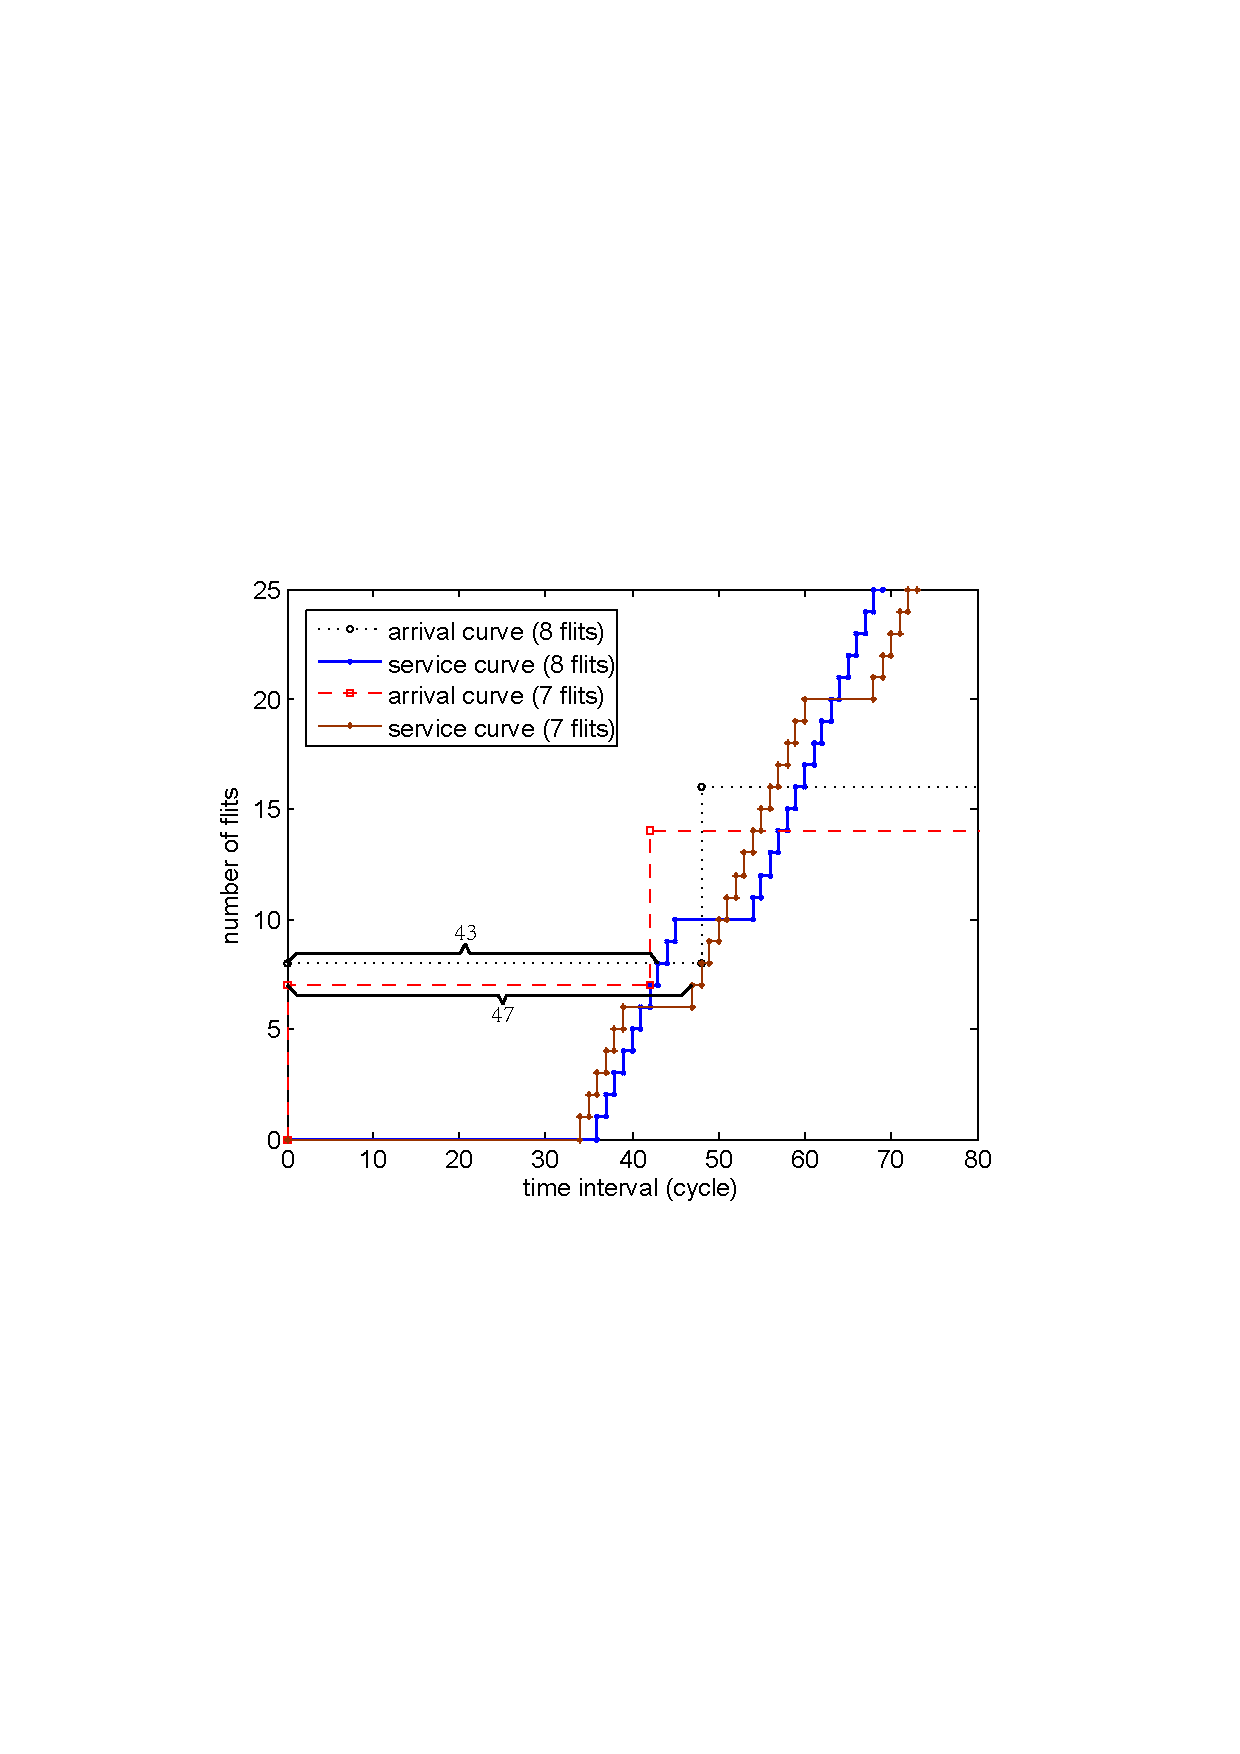
\includegraphics[scale=0.63]{figures/reason.pdf}\\
  \caption{Delay Comparison between $F_i=7$ and $F_i=8$}\label{reason}
\end{figure}

\subsection{Comparison with Simulation}\label{sim}
The correctness of our delay analysis algorithm and buffer sizing algorithm is verified by simulation. We modified the Booksim 2.0 simulator \cite{6557149} to support the specified traffic pattern and injection process. Examples investigated in this section include the traffic pattern shown in Fig. \ref{topology} and a real application provided by Ericsson Radio Systems and discussed in \cite{LuJa08}\cite{Jafari1922089}. We adopt the optimized lookahead pipeline router  \cite{jerger2009chip} to construct the mesh network presented in Fig. \ref{topology}, which remove the RC stage from the pipeline. Our service model is customized to fit this optimization by letting the service curve of RC stage be $\delta_0(t)$. Other architecture and simulation parameters are listed in the Table \ref{arcpara}.
\begin{table}[htbp]
\centering
\caption{\label{arcpara}Architecture parameters used in the simulation}
\begin{tabular}{|c|c||c|c|}
\hline
network topology    & $4\times 4$ mesh  &   routing algorithm & X-Y routing\\
\hline
clock cycle   & 1 ns &   channel width   & 128 bits\\
\hline
buffer size &   16 flits  &   switch allocator    &   priority-aware\\
\hline
VC allocator    &   reserved    & sampling period &   $1\times 10^5$ cycles\\
\hline
credit delay &  1 cycle   &  warmup period  & $1\times 10^5$ cycles \\
\hline
\end{tabular}
\end{table}

For the traffic pattern shown in Fig. \ref{topology}, we set the injection rate $V_i$ to $1/6$ flits/cycle, and change the packet length from two flits to nine flits. The collected maximum end-to-end delay of the four flows obtained by simulation and our RTC method is shown in Fig. \ref{rtcvssim}. To prevent the results of flow $f_2$ from shading the results of $f_3$, we exchange the order of $f_3$ and $f_4$ in this figure. As indicated in the comparison, for the given configuration, delay calculated with our method is indeed an upper bound of the simulation results, which verifies the correctness of our methods. In addition, we also found that, the delay bound of high-priority flows (e.g. $f_1$ and $f_4$) is tighter than that of low-priority flows.
\begin{figure}
  \centering
  % Requires \usepackage{graphicx}
  \includegraphics[scale=0.8]{figures/rtcvssim.pdf}\\
  \caption{Comparison with simulation}\label{rtcvssim}
\end{figure}

We also take the real application discussed in \cite{LuJa08}\cite{Jafari1922089} as an example to demonstrate the accuracy and ability to analyze multi-flows. This application is comprised of 16 IP cores. The 26 communication flows among these 16 IPs are classified into nine groups, and each group has their bandwidth requirement. When mapped to a $4\times 4$ mesh network, the traffic pattern of this application is demonstrated in Fig. \ref{trafficpattern}(a). We assume the flows in a group have the same injection period and priority. The flow specification of each group is listed in Table. \ref{trafficpattern}(b). We set the packet size to 128 bits, and collect the end-to-end delay of each flow obtained by simulation and our method, the related results is shown in Fig. \ref{ericsson}. We can see that the calculated results constrain the simulation results well, which verifies the correctness of our method.
\begin{figure}
  \centering
  % Requires \usepackage{graphicx}
  \includegraphics[scale=0.7]{figures/trafficpattern.pdf}\\
  \caption{Traffic pattern of ericsson radio system application}\label{trafficpattern}
\end{figure}

\begin{figure*}
  \centering
  % Requires \usepackage{graphicx}
  \includegraphics[scale=0.45]{figures/ericsson.pdf}\\
  \caption{Comparison with simulation}\label{ericsson}
\end{figure*}

\section{Conclusion}\label{conclusion}
The priority-aware wormhole-switched NoC is a promising platform for the on-chip real-time communication if the worst-case performance can be accurately analyzed and guaranteed. Simulation is not well suited for this purpose because it is difficult to cover all the corner cases. In this paper, we propose an RTC based performance model to achieve this goal. We first build the traffic model and service model for this NoC, and propose a novel method to derive the upper service curve of credit-based flow control. Compared with the FLA and LLA methods which assume the router to be single cycle and free of flow control, our performance model is more general and comprehensive. Based on the proposed RTC model, we then proposed an end-to-end delay analysis algorithm and a buffer sizing algorithm. The delay analysis algorithm can be implemented to compute the end-to-end delay for each flow automatically, and verify whether all these flows meet their deadline under this configuration. The proposed buffer sizing algorithm can optimize the buffer size from high-priority flows to low-priority flows. It can also be implemented to perform the buffer reduction automatically under the constraint of deadline. Compared with the DNC based performance model, our model can give tighter performance bound, because the RTC-based model takes the upper service curve and lower arrival curve into consideration. Experimental results also illustrate that our method indeed outperforms the conventional analytical methods, e.g. LLA and DNC, when the tightness of performance bound are considered. Our results can be applied to the mapping, routing and power reduction of NoC.

\section*{Acknowledgement}
The authors thank the reviewers for their suggestions and comments, and all the experiments are carried out at the Integrated Microsystem Lab (IML) of McGill University. The first author also thank Ari Ramdial at McGill University for his helpful comments. This research is supported by High Technology Research and Development Program of China (Grant No. 2012AA012201, 2012AA011902).


\section*{References}

\bibliography{Docear}

\end{document} 